\documentclass{sigchi}

% Use this section to set the ACM copyright statement (e.g. for
% preprints).  Consult the conference website for the camera-ready
% copyright statement.

% Copyright
\CopyrightYear{2016}
%\setcopyright{acmcopyright}
\setcopyright{acmlicensed}
%\setcopyright{rightsretained}
%\setcopyright{usgov}
%\setcopyright{usgovmixed}
%\setcopyright{cagov}
%\setcopyright{cagovmixed}
% DOI
\doi{http://dx.doi.org/10.475/123_4}
% ISBN
\isbn{123-4567-24-567/08/06}
%Conference
\conferenceinfo{CHI'16,}{May 07--12, 2016, San Jose, CA, USA}
%Price
\acmPrice{\$15.00}

% Use this command to override the default ACM copyright statement
% (e.g. for preprints).  Consult the conference website for the
% camera-ready copyright statement.

%% HOW TO OVERRIDE THE DEFAULT COPYRIGHT STRIP --
%% Please note you need to make sure the copy for your specific
%% license is used here!
% \toappear{
% Permission to make digital or hard copies of all or part of this work
% for personal or classroom use is granted without fee provided that
% copies are not made or distributed for profit or commercial advantage
% and that copies bear this notice and the full citation on the first
% page. Copyrights for components of this work owned by others than ACM
% must be honored. Abstracting with credit is permitted. To copy
% otherwise, or republish, to post on servers or to redistribute to
% lists, requires prior specific permission and/or a fee. Request
% permissions from \href{mailto:Permissions@acm.org}{Permissions@acm.org}. \\
% \emph{CHI '16},  May 07--12, 2016, San Jose, CA, USA \\
% ACM xxx-x-xxxx-xxxx-x/xx/xx\ldots \$15.00 \\
% DOI: \url{http://dx.doi.org/xx.xxxx/xxxxxxx.xxxxxxx}
% }

% Arabic page numbers for submission.  Remove this line to eliminate
% page numbers for the camera ready copy
% \pagenumbering{arabic}

% Load basic packages
\usepackage{balance}       % to better equalize the last page
\usepackage{graphics}      % for EPS, load graphicx instead 
\usepackage[T1]{fontenc}   % for umlauts and other diaeresis
\usepackage{txfonts}
\usepackage{mathptmx}
\usepackage[pdflang={en-US},pdftex]{hyperref}
\usepackage{color}
\usepackage{tabularx, booktabs}
\usepackage{textcomp}
\usepackage{subcaption}
\usepackage{graphicx}
\usepackage[toc,page]{appendix}
\usepackage[inline]{enumitem}
\usepackage{float}
\usepackage{csquotes}

% Some optional stuff you might like/need.
\usepackage{microtype}        % Improved Tracking and Kerning
% \usepackage[all]{hypcap}    % Fixes bug in hyperref caption linking
\usepackage{ccicons}          % Cite your images correctly!
% \usepackage[utf8]{inputenc} % for a UTF8 editor only

% Packages
\usepackage[table,xcdraw]{xcolor}
\usepackage{enumitem}
%\usepackage{booktabs,caption}
\usepackage{tabularx}
\usepackage[flushleft]{threeparttable}

% Custom column type for tabularx environment. Centers and fills
\newcolumntype{Y}{>{\centering\arraybackslash}X}
\newcolumntype{Z}{>{\raggedleft\arraybackslash}X}
\newcolumntype{W}{>{\raggedright\arraybackslash}X}

% Paper metadata (use plain text, for PDF inclusion and later
% re-using, if desired).  Use \emtpyauthor when submitting for review
% so you remain anonymous.

\def\plaintitle{The relationship between tap pressure on pressure sensitive touchscreens and the users's emotional state}
\def\plainauthor{First Author, Second Author, Third Author,
  Fourth Author, Fifth Author, Sixth Author}
\def\emptyauthor{}
\def\plainkeywords{Human centered multimedia; emotion; tap pressure; motor expression}
\def\plaingeneralterms{Documentation, Standardization}

% llt: Define a global style for URLs, rather that the default one
\makeatletter
\def\url@leostyle{%
  \@ifundefined{selectfont}{
    \def\UrlFont{\sf}
  }{
    \def\UrlFont{\small\bf\ttfamily}
  }}
\makeatother
\urlstyle{leo}

% To make various LaTeX processors do the right thing with page size.
\def\pprw{8.5in}
\def\pprh{11in}
\special{papersize=\pprw,\pprh}
\setlength{\paperwidth}{\pprw}
\setlength{\paperheight}{\pprh}
\setlength{\pdfpagewidth}{\pprw}
\setlength{\pdfpageheight}{\pprh}

% Make sure hyperref comes last of your loaded packages, to give it a
% fighting chance of not being over-written, since its job is to
% redefine many LaTeX commands.
\definecolor{linkColor}{RGB}{6,125,233}
\hypersetup{%
  pdftitle={\plaintitle},
% Use \plainauthor for final version.
%  pdfauthor={\plainauthor},
  pdfauthor={\emptyauthor},
  pdfkeywords={\plainkeywords},
  pdfdisplaydoctitle=true, % For Accessibility
  bookmarksnumbered,
  pdfstartview={FitH},
  colorlinks,
  citecolor=black,
  filecolor=black,
  linkcolor=black,
  urlcolor=linkColor,
  breaklinks=true,
  hypertexnames=false
}

% create a shortcut to typeset table headings
% \newcommand\tabhead[1]{\small\textbf{#1}}

% End of preamble. Here it comes the document.
\begin{document}

\title{\plaintitle}

\numberofauthors{1}
  \author{
  \alignauthor Kevin Blom\\
         \affaddr{University of Amsterdam}\\
         \affaddr{Science Park 904}\\
         \email{kevin.a.blom@gmail.com}
  }
\maketitle

\begin{abstract}
  % UPDATED---\today. This sample paper describes the formatting
  % requirements for SIGCHI conference proceedings, and offers
  % recommendations on writing for the worldwide SIGCHI
  % readership. Please review this document even if you have submitted
  % to SIGCHI conferences before, as some format details have changed
  % relative to previous years. Abstracts should be about 150 words and
  % are required.
The detection of emotion has been a subject of research for a long time and is key to affective computing; computers that assist humans or have an enhanced decision ability based on the user. One of the areas that recently has become available is pressure sensitive touchscreens. Touchscreens are a widely accepted and used technology where users deliberately interact with multiple times per day. This study tries to predict emotion from tap pressure by using a pressure sensitive touchscreen and an affective picture database. Unfortunately, while literature does suggest a correlation, this study finds none, $p > .05$. Additionally, a small study is performed to explore a relationship between tap pressure and tap duration, which does show significance, $p < .0005$ The discussion raises some weaknesses as to the cause and proposes several solutions for further investigation.
\end{abstract}

\category{H.5.2.}{Information Interfaces and Presentation}{User-centered design}

\keywords{\plainkeywords}

\begin{displayquote}
\quad
\begin{flushleft}
\small
\textbf{Theodore}: \textit{Are you in love with anybody else?}\\
\textbf{Samantha}: \textit{Why do you ask that?}\\
\textbf{Theodore}: \textit{I do not know. Are you?}\\
\textbf{Samantha}: \textit{I've been thinking about how to talk to you about this.}\\
\textbf{Theodore}: \textit{How many others?}\\
\textbf{Samantha}: \textit{641.} 
\end{flushleft}

\begin{flushright}
\textit{Her (2013) } 
\end{flushright}
\end{displayquote}

\section{Introduction} % (fold)
\label{sec:introduction}

Reeves et al. \cite{Reeves1998} have shown that humans have the unconscious and unintentional response to computers to act in a natural and social way. Lindstrom \cite{Lindstrom2011} used an MRI machine to show that the parts of the brain that are active when in love are the same parts that are active when someone hears their smartphone ring. It tells us that users literally \textit{love} their smartphone. 

Emotion aware smart devices can provide users with a better experience, where better can be classified as an experience in line with how the user is feeling. Screens and information that present themselves in different ways, where the differences originate from current feelings of the user. Picard \cite{Picard1995} states that computers that are emotion aware not only possess the ability to be of the users' assistance but also let that computer make decisions that are influenced by those emotions that are expressed by the user. This type of adaptation of user interfaces and information can tighten the social bond between user and smart devices making the devices feel more alive. Furthermore, the current state of technology, and in particular machine learning, is capable of using the emotion of users in product designs that dynamically change. If users love the smartphones in their pockets, why not try to make those small computers respond in a natural, social way, making them feel more alive?

However, as Zimmerman et al. \cite{Zimmermann2003} note in their conclusion: What are adequate emotional reactions of a system that knows how the user feel? One possibility could be that a telecom provider app or website can contact customer support in the background already when it notices the user is upset about their bill. Another interesting case would be music applications promoting new and exciting songs when the user is happy, but slowed down and calm songs when the user is relaxed. Alternatively, games that have characters that can be helpful and friendly when progression is stalling, but can also suitably respond to aggression and anger, mitigating frustration or escalation. As a final example, educational systems that can detect if the user is confused can provide additional examples, or when it notices boredom can provide more challenging exercises.

The field where this study fits in is called affective computing. It concerns itself with computers that have the means to detect, respond, and express emotion. The goal of this study is more specific, it will be within the field of emotion detection of computers and explores the use of pressure sensitive touchscreens of smart devices as means for a less intrusive, more ubiquitous and less intrusive way of detecting emotion.

Further reading of this section is divided into four parts; models of emotion, measuring of emotion, practical and applied applications, and research question and hypotheses. Models of emotion will help to grasp the different ways to approach and classify emotions, whereas measuring of emotion will help understand how measuring is currently executed and how it can be improved. Subsequently, several applied applications are discussed in order to explore the existing landscape of emotion detection in practice. Finally, before moving on to the methods, a research question and a hypothesis are presented.

\subsection{Models of emotion} % (fold)
\label{sub:models_of_emotion}
There exist several different models of emotion that attempt to classify human emotion in varying ways. In 2000, Scherer \cite{scherer2000} presents four models to represent emotion:
\begin{enumerate*}[label=(\alph*)]
  \item dimensional,
  \item discrete emotion,
  \item meaning, and
  \item componential.
\end{enumerate*}
Their focus lies respectively with subjective feeling, motor expression and adaptive behavior patterns, verbal descriptions of subjective feelings, and the link between emotion-antecedent evaluation and differentiated reaction patterns. The study tries to name often used elicitation mechanisms; however, it fails to find specific mechanisms for all but the componential model, which often uses an appraisal mechanism. Appraisal is one of the six components that Fontaine et al. \cite{Fontaine2007} incorporate in their model of emotions. The complete model that they present consists of six components:
\begin{enumerate*}[label=(\alph*)]
  \item appraisals of events
  \item psychophysiological changes,
  \item motor expressions,
  \item action tendencies,
  \item subjective experiences, and
  \item emotion regulation.
\end{enumerate*}

\begin{figure}[t]
    \centering
    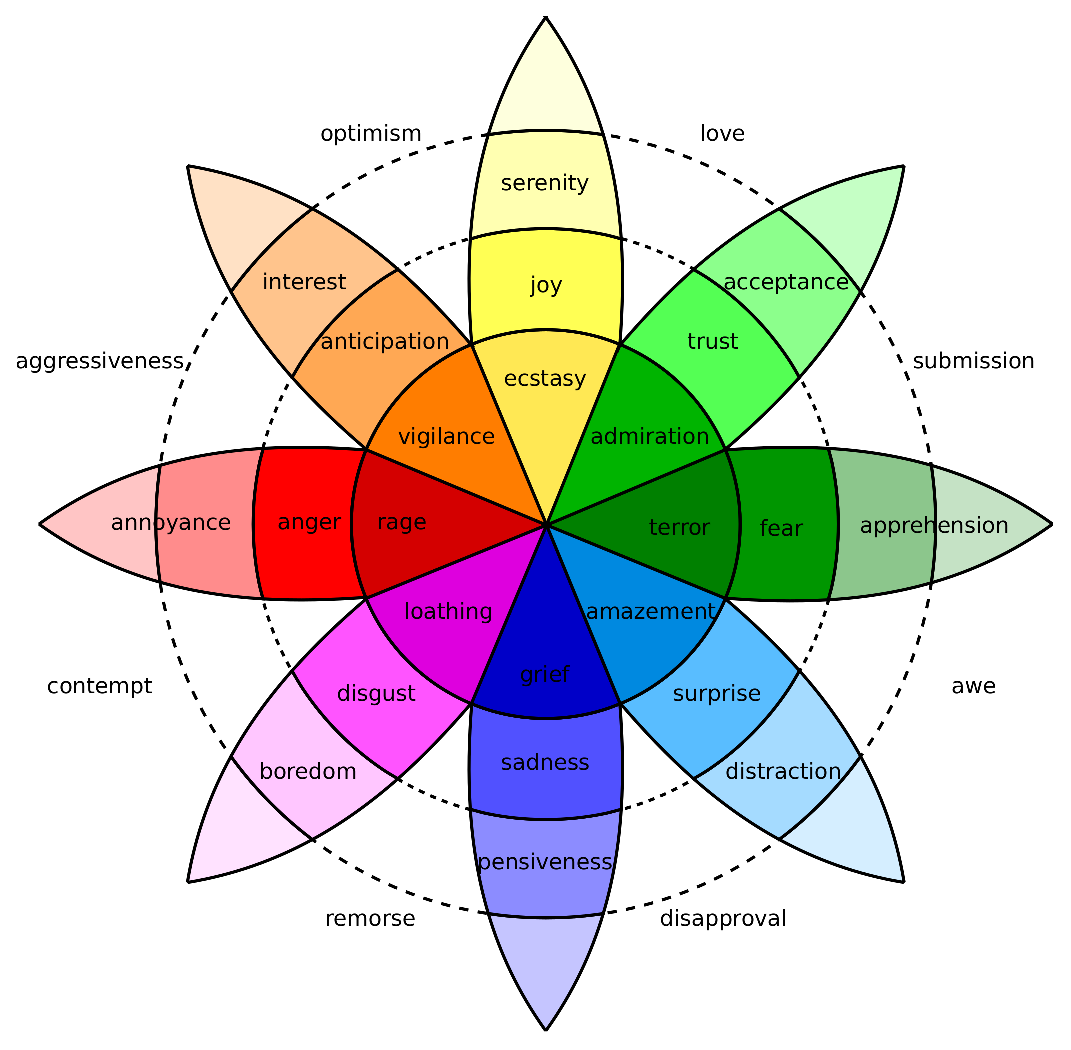
\includegraphics[width=0.45\textwidth]{images/PlutchikWheelOfEmotions.eps}
    \caption{The discrete three dimensional model that R. Plutchik \protect\cite{Plutchik1980} introduced in 1980. It shows human emotions on a discrete scale, where the most intense emotion is displayed in the middle, and intensity drops when going outwards.}
    \label{fig:wheel_of_emotions}
\end{figure}

More recently, Shah et al. \cite{Shah2015} state that there are in general two directions to represent emotion; discrete and continuous. The discrete model represents emotions that are measurable and physiologically distinct like angry, sad, happy, and others \cite{Ekman1992}. A more detailed discrete model is the one proposed by Plutchik \cite{Plutchik1980}. The continuous model represents emotions on a two-dimensional scale, where one axis represents \textit{valence} and the other \textit{arousal} \cite{Posner2005} (Figure \ref{fig:circumplex_model}). Mauss et al. \cite{Mauss2009} suggest that using a dimensional, continuous framework is a better option when capturing emotion, relative to discrete frameworks. 

\begin{figure}[ht]
    \centering
    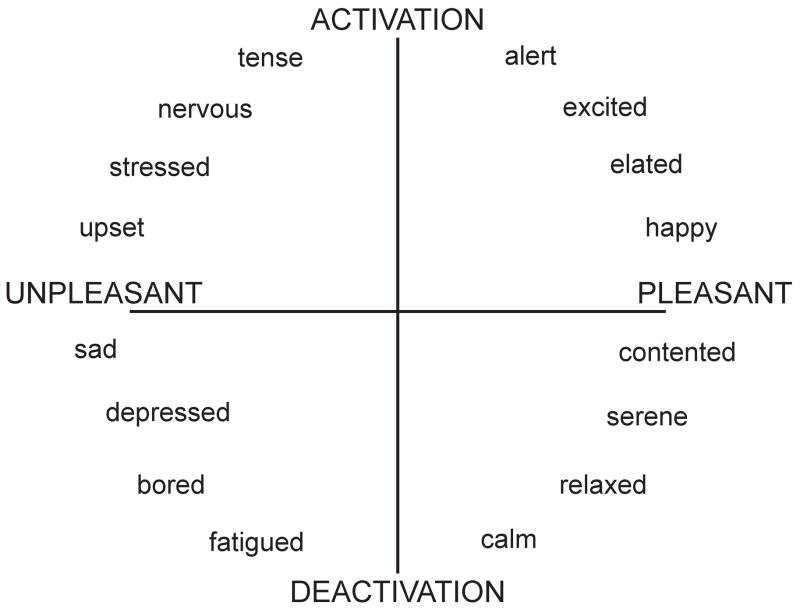
\includegraphics[width=0.45\textwidth]{images/CircumplexModel.jpg}
    \caption{The two dimensional model as explained by Posner et al. \protect\cite{Posner2005}. Valence is expressed on the x-axis, arousal on the y-axis. Rather than classifying each emotion discretely, it can put emotion anywhere on the two axes}
    \label{fig:circumplex_model}
\end{figure}

\subsubsection{Physiological detection} % (fold)
\label{sub:physiology}
The first domain uses physiological signals of the human body to measure and detect emotion. In a review by Wioleta\cite{Wioleta2013}, eight studies were collected that measure emotion using one or more physiological signals combined. These signals are (in no particular order):
\begin{enumerate*}[label=(\alph*)]
  \item EEG,
  \item skin conductance,
  \item blood volume pulse,
  \item temperature,
  \item heart rate,
  \item blood pressure,
  \item respiration,
  \item EMG, and
  \item ECG.
\end{enumerate*}
Most of these physiological signals have the drawback that they need specialized sensors attached to the body, making unobtrusive measurements difficult. With the recent rise of smart wearables that include a heart rate monitor, heart rate is one of the signals that is more readily available to use in applications on smart devices.
% subsection physiology (end)

\subsubsection{Facial detection} % (fold)
\label{sub:facial_detection}
Facial detection of emotion incorporates the measurement of facial muscle movement, voice or speech \cite{Ververidis2004}, and furthermore includes the eye as point of detection, i.e. movement, blinking, and pupil dilation \cite{Soleymani2015}. While one can argue that these methods are also physiological, they are researched to such detail and extent that they can be classified separately. By connecting facial muscle movement to the visual display of emotions, Ekman et al. \cite{Ekman1969} conclude with a core set of six mutually exclusive emotions that could be recognized. Furthermore, De Silva et al. \cite{Silva1997} found that several emotions are expressed by either visual or auditory cues, or both, meaning that some emotions can be recognized by visual cues alone, auditory cues alone, or need a combination of both to be detected accurately.
% subsection facial_emotion_detection (end)

\subsubsection{Posture/gestures emotion detection}
Other means of detection emotions involve the tracking and interpretation of posture and gesture. Wallbott et al. \cite{Wallbott1998} concluded in 1998 that there are, in some cases, distinctive patterns of movement and postural behavior that have a strong correlation to emotions. In other cases, they mention that in the absence of patterns there are still distinctive features from which emotion can be inferred. Coulson et al. \cite{Coulson2004} researched static body postures and the recognition of emotions from these body postures by participants. It showed that disgust is a tough emotion to recognize but anger and sadness had over 90\% correct detection rates. Furthermore, they conclude that happiness and surprise were two emotions that were often confused. 
% subsection measuring_emotion (end)

\subsection{Applied emotion and pressure detection} % (fold)
\label{sub:practical_applications}
First, Hertenstein et al. \cite{Hertenstein2006} show that touch can communicate distinct emotions. Looking at the more practical and applied side of emotion detection, Gao et al. \cite{Gao2012} used touchscreen devices, where the application of gestures on touchscreens is successfully linked to emotional states with the use of a game. The emotional states that were tested for are: excited, relaxed, frustrated and bored, and accuracy of detection reached at minimum 69\%. However, the research of Gao et al. was limited to gestures and did not incorporate data from taps. Furthermore, Lv et al. \cite{H.R.LvZ.L.LinW.J.Yin2008} have created means to detect emotion from keyboard pressure using feature extraction. This indicates that the use of a keyboard on a touchscreen could also be used as means of detecting emotion, but one must keep in mind that a regular keyboard is not entirely comparable to a touchscreen keyboard. It lays flat on a desk and is often typed upon with more than one or two fingers, which means that the pressure exerted on the keyboard is likely not directly correlated with the pressure on a touchscreen keyboard. Moreover, Lee et al. \cite{Lee2012} propose an unobtrusive way of detecting emotion by analyzing smartphone usage patterns (not unlike LiKamWa et al. \cite{Likamwa2013}) and social network status updates. However, this required that the user would post status updates through independently developed social networking applications, that are not officially supported by the social networks themselves and which could possibly invade privacy. Gr{\"{u}}nerbl et al. \cite{Grunerbl2015} employ a smartphone and sensor fusion to detect 17 emotional states and state changes in bipolar disorder patients. Utilizing pattern recognition of phone call features, speech features, GPS data, and accelerometer data, 76\% recognition accuracy is reached. This study did not use invasive body sensors but does use data of (amongst others) phone calls like unique numbers dialed, the average length of phone calls, and percentage of speaking in the whole conversation. This is privacy sensitive data that is analyzed for emotion detection. Essl et al. \cite{Essl2010} have studied touch-width based force-like sensing using the Android API for musical instruments. It infers touch pressure based on the total surface area of a finger that touches the screen, and the approach by Essl et al. resulted in four distinct pressure levels using only built-in sensors of a smartphone. Goel et al. \cite{Goel2012} developed GripSense, another way to continuously detect pressure rather than a one-time approximate detection as Essl et al. performed. By using the vibration motor and gyroscope in a smartphone, three distinct pressure levels could be detected with a 95.1\% accuracy.

% subsection practical_applications (end)

\subsection{Research question and hypotheses}
From the reviewed literature it can be concluded that measuring emotion often requires invasive sensors attached to the body to measure various physiological signals, invades privacy by constantly analyzing camera images or microphone signals, or requires the user to execute specific actions like playing a game or entering text. The practical applications show one thing in common: a touchscreen. The touchscreen is a technology many people interact with every day, where they deliberately choose to participate in those interactions and is independent of a use case if the user does not need to access a specific app or website. Using touchscreen presses as indicators for an emotional state could be an unintrusive way of detecting emotion without the need for constant monitoring through other sensors. With the introduction of pressure sensitive touchscreens in recent smart devices, an interesting new sensor is added to the plethora of sensors already available, which leads to the following research question:\\

\textit{Can pressure sensitive touchscreen devices be used to tell more about the emotional state of the user?}\\

The presented research question prompts thorough investigation of the connection between the pressure that a tap exerts on a touchscreen and the emotional state of the user that performs the taps. It sets the scope of the study to motor expression analysis, one of the six components mentioned by Fontaine et al. \cite{Fontaine2007}. The null hypothesis that springs from the research question is:

$H_0$: \textit{Pressure of taps on touchscreens exhibit no correlation with emotional state.}
\\\\and the alternative hypothesis:\\\\
$H_1$: \textit{Pressure of taps on touchscreens exhibit direct correlation with emotional state.}

Furthermore, the data that is collected during the experiment allows for a smaller study besides the main research question. It concerns the relationship of tap pressure and tap duration. Interest for this smaller study stems from the unavailability of pressure sensitive touchscreens. They have become more common, but only one major smartphone manufacturer utilizes them. If tap pressure and tap duration show a relationship, it indicates that any touchscreen can be used for predicting tap pressure without the need for pressure sensitive touchscreens. The next section will present how the study was conducted before it continues to present the results.

% \begin{itemize}
%   \item Description of background.
%   \item Explanation of why research was necessary.
%   \item Description of how research will be undertaken.
% \end{itemize}

% section Introduction (end)

\section{Methods} % (fold)
\label{sec:methods}
In order to test for the correlation between taps on a touchscreen and emotion, there has to be a standardized way of eliciting different emotions and a measurement plan for tap pressure. Besides explaining the methods for the main study, this section also explains the methods of the beforementioned smaller, second study that will explore a relationship between tap pressure and tap duration. For this experiment, 51 Participants were selected using a convenience sampling process at an office. The participants varied in age, educational level, current line of work, and background. 

\subsection{Emotional elicitation} % (fold)
\label{sub:emotional_elicitation}
For the experiment, a standardized photographic test image set has been used that often has been used succesfully for measuring emotional response of viewers. This photo set measured emotional response a two-dimensional valence and arousal scale and is called the Geneva Affective Picture Database \cite{Dan-glauser2011}. Utilizing the emotional responses elicited by this photo set as a baseline, touchscreen taps and their pressure can be compared to the emotional response. The photo set counts 730 pictures and is divided into six categories: Animal, Human, Neutral, Positive, Snakes, Spiders. From each of the categories, ten pictures were randomly selected, resulting in a set of 60 pictures used for the experiment. Each participant was presented with the same 60 pictures, but in random order in order to mitigate any side effects that might occur from presenting pictures in a particular order. Brown et al. \cite{Neuroscience2012} remark that 5-second exposure to pictures is often used for the IAPS (International Affective Picture System) \cite{Lang1997} photos. The GAPED photo set has been created because of two issues with the IAPS; extensive use decreases the impact of the stimuli and the limited number of pictures for specific themes. Both these issues are not exposure time related, so the choice of exposure time of the photo to the participant is five seconds.

% subsection emotional_elicitation (end)

\subsection{Pressure detection} % (fold)
\label{sub:pressure_detection}
Taps were detected on an Apple iPhone 6s device with a 3D touchscreen running iOS 10.3.1. The pressure of taps was registered on a floating point scale from 0.0 to 6.67 (Corresponding with 0 to $\pm$350 grams). For every tap, several pressure measurements were registered in chronological order. Furthermore, the duration of a tap (in nanoseconds) was recorded.
% subsection pressure_detection (end)

\subsection{Data collection} % (fold)
\label{sub:data_collection}
In order to collect a larger data set, four taps per photo were required to advance to the next photo. These taps are directed with the use of gray colored buttons that are randomly shown on a four by four grid on the screen (Figure \ref{fig:grid}). The random pattern of the buttons ensures that the position of the tap on the screen does not matter for the pressure measurement once the tap pressures are averaged. It uses a gray color because it is perceived as neutral. The buttons are random for every photo, and for every participant. In other words, no participant received the same grid for the same photo.
\begin{figure}[t]
    \centering
    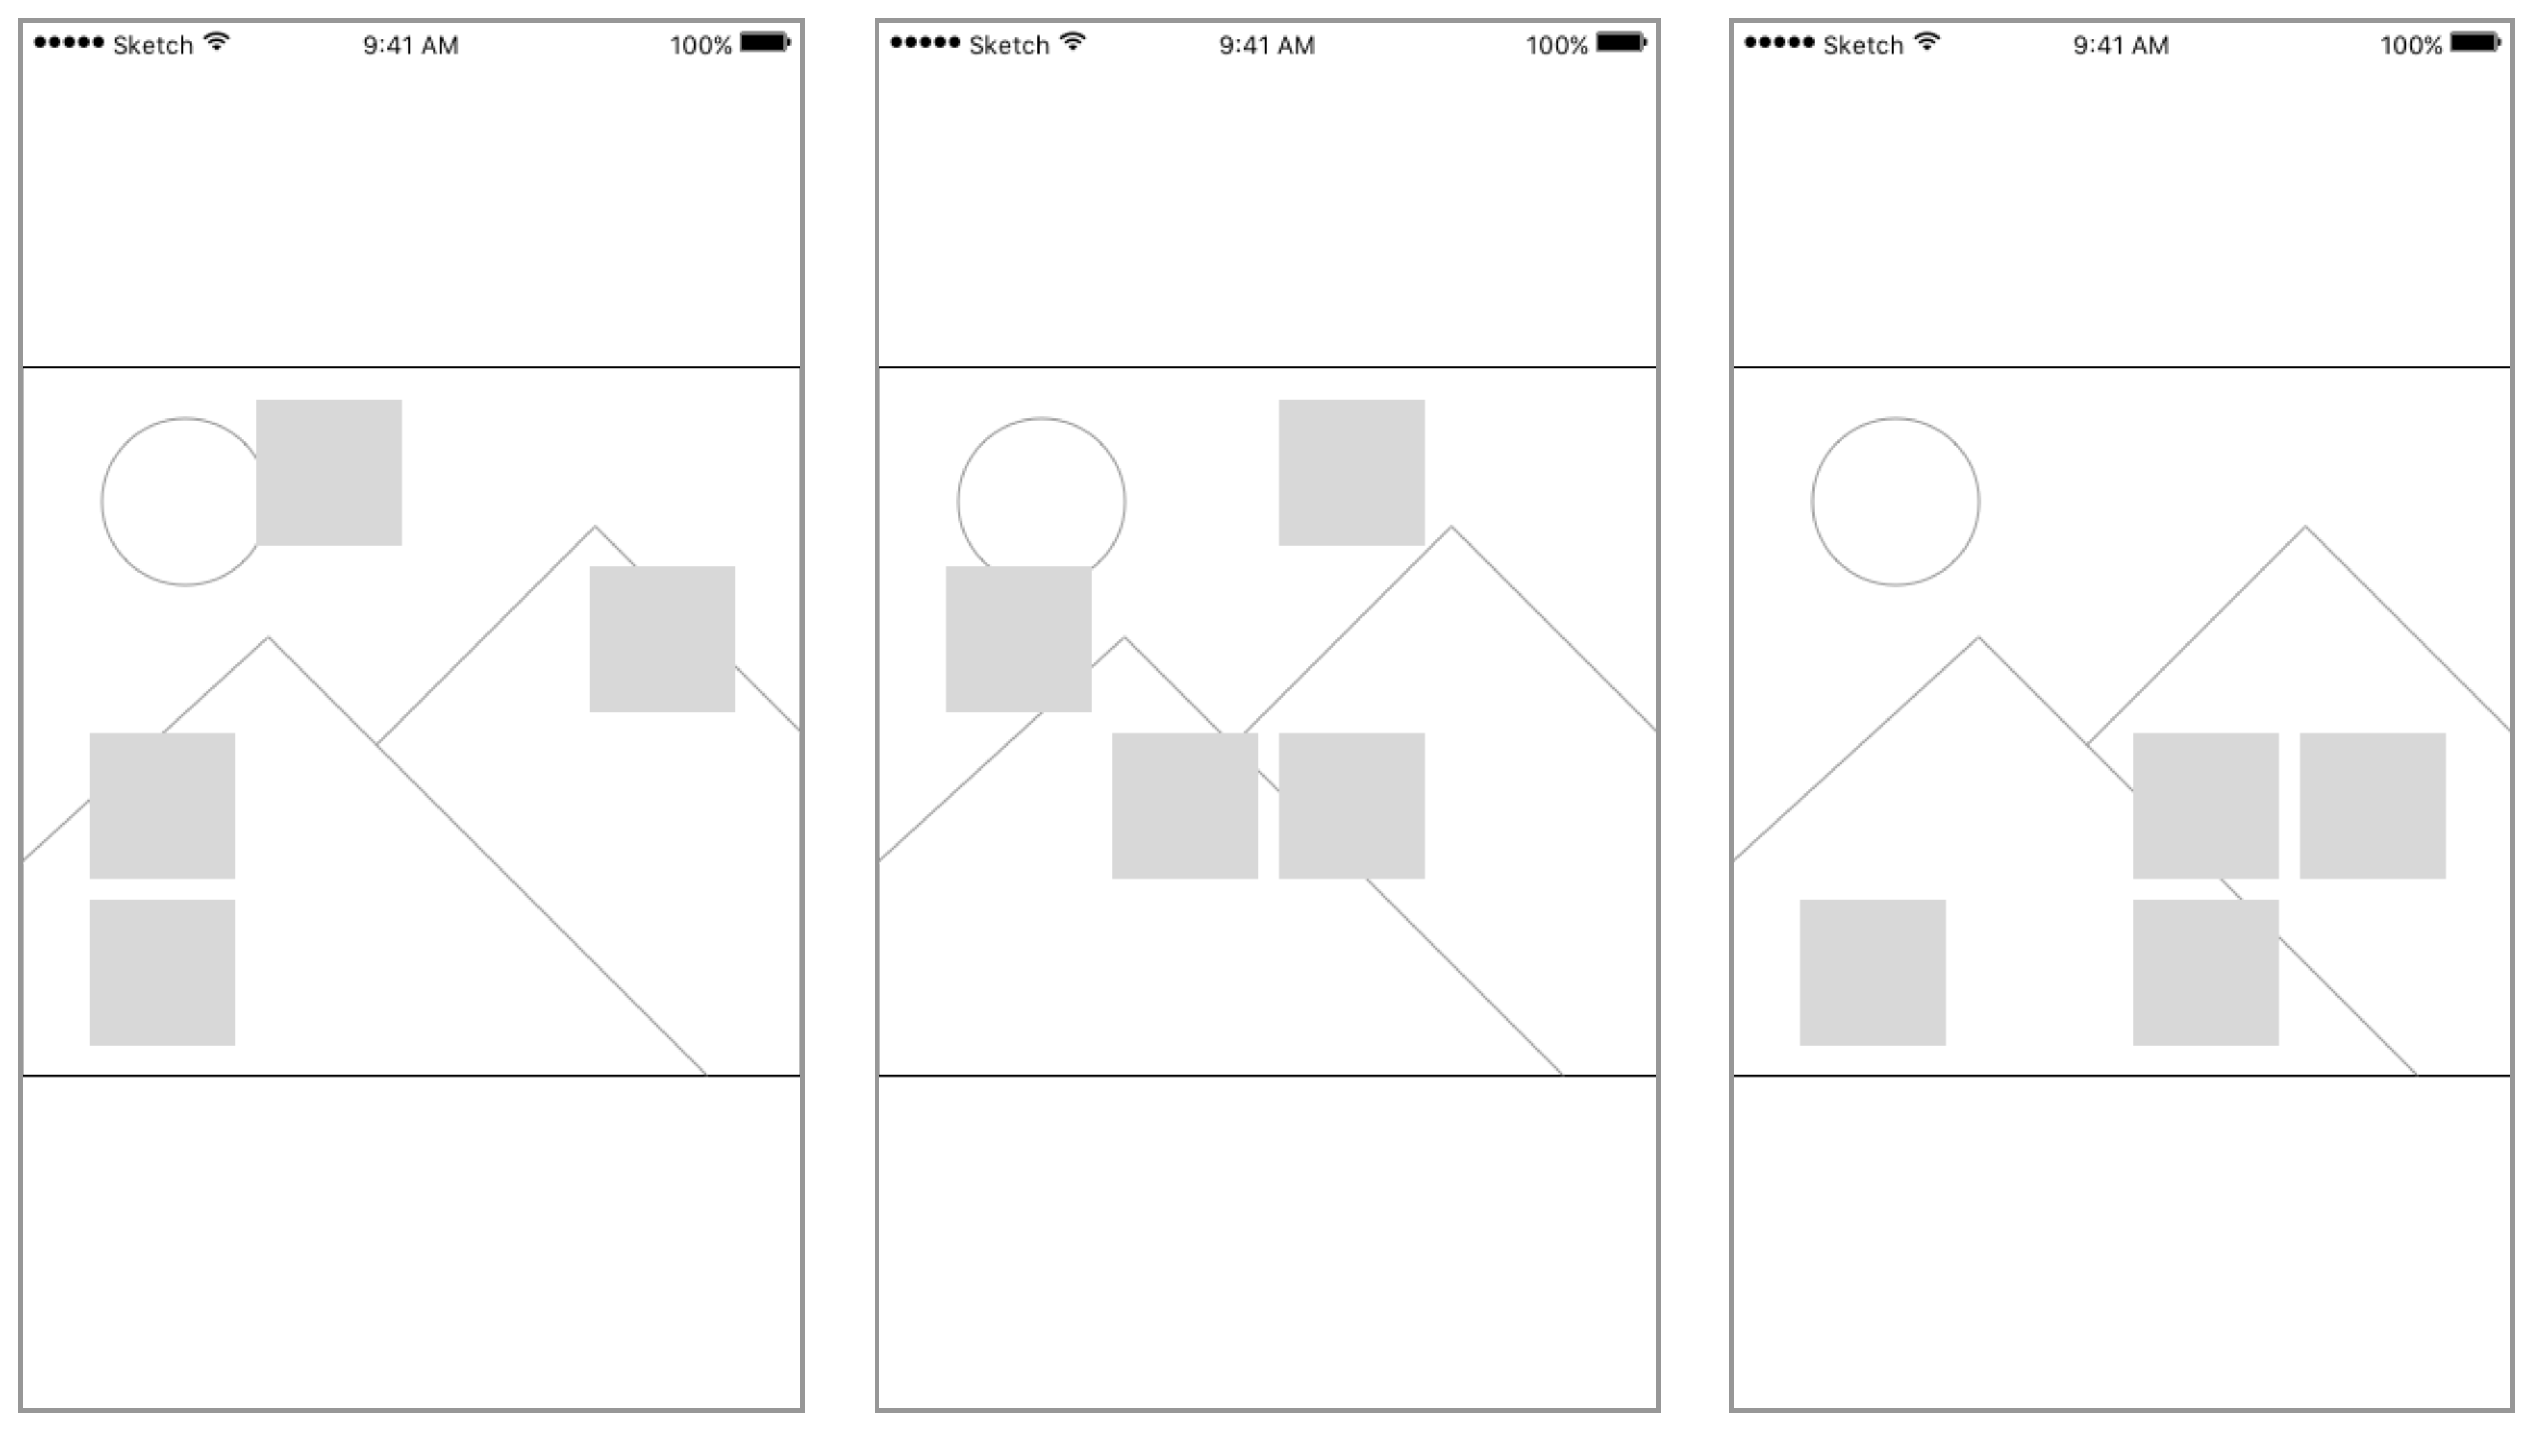
\includegraphics[width=0.46\textwidth]{images/Grid.eps}
    \caption{Three examples of the grid as presented over a picture shown on a smartphone. When a participant has pressed each of the gray squares (which disappear when pressed upon) the next picture is shown. After five seconds a new randomly generated grid is displayed on top of the picture. This process repeats 60 times.}
    \label{fig:grid}
\end{figure}

All the data that was collected was anonymously and securely sent real-time to a Firebase \cite{google:firebase} database. Firebase utilizes a JSON \cite{json} tree structure that is described in Figure \ref{fig:datastructure}. The figure also provides are more detailed look into which data was collected and the experiment setup.
\begin{figure}[t]
    \centering
    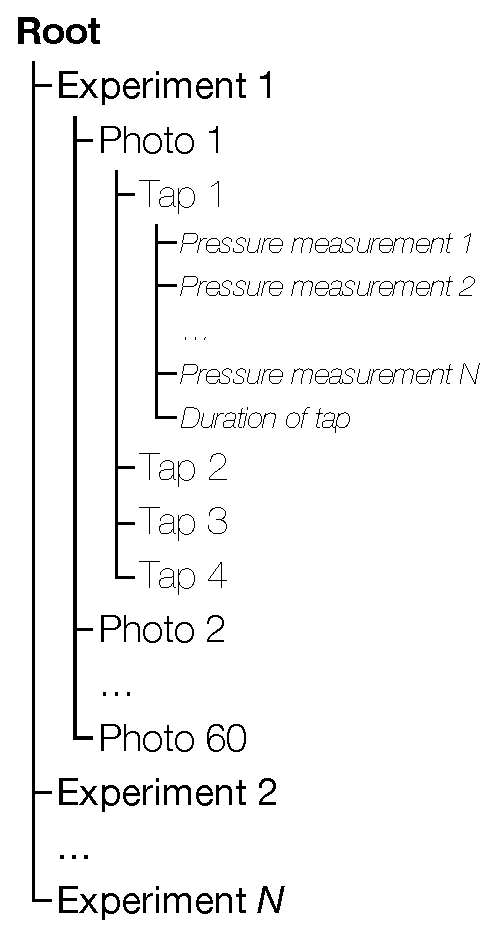
\includegraphics[width=0.25\textwidth]{images/Datastructure.eps}
    \caption{The database structure shows that for every experiment entry, there are 60 photo entries. Each photo entry contains four tap entries, that contain zero to \textit{n} pressure measurements and a duration measurement.}
    \label{fig:datastructure}
\end{figure}

% subsection data_collection (end)

\subsection{Experiment setup} % (fold)
\label{sub:experiment_setup}
Firstly, participants were informed about what the experiment entailed and were presented with a consent form. Subsequently, the participants continued the experiment on the smart device with a test application. The entirety of the experiment was completed in a room that contained no screens, speakers or other distractions, otherwise known as the 'Zen room', and ensured the participants were focused on the experiment. The test application was structured as follows:
\begin{enumerate}
  \item The participant is presented with a screen that asks if they received and signed a consent form and if not, that they should contact the supervisor immediately. There is also a \textit{start} button to start the experiment.
  \item If the participant pressed the \textit{start} button, the first picture is shown.
  \item After five seconds, four gray buttons are shown, overlaid on the picture in a random pattern (Figure \ref{fig:grid}).
  \item When the participant pressed all the four buttons, the next picture is presented.
  \item This process repeats until all 60 pictures were shown.
  \item The participant is presented with a final screen that contains a thank you message and refers to the supervisor if there are questions.
\end{enumerate}

When the experiment had concluded, participants were informed about the nature of the experiment (i.e. they were informed of the research question) and any questions they asked were answered.
% subsection experiment_setup (end)

\subsection{Data analysis}
\label{sub:data_analysis}
The collected data was exported as JSON from Firebase and subsequently mutated using Python 2.7 \cite{python} on macOS 10.12.4 \cite{macOSSierra} in order to create an \textit{.csv} file that was readable by SPSS 24.0.0.0 \cite{SPSS}. Because of a suspicion that either maximum exerted pressure or average exerted pressure of a tap might be of influence, these two variables were manually added using averaging. For maximum pressure, the maximum pressure value of each tap was extracted, and for each photo, this was averaged. Regarding average tap pressure, the average pressure of a tap was calculated and subsequently, all the average tap pressures were averaged again per photo. These averages make it possible to compare means. The result is six variables in SPSS; 
\begin{enumerate}
  \item \textbf{Photo filename} - String, containing the photo filename for identification purposes.
  \item \textbf{Valence} - Numeric, decimal value on a scale from 0.0-100.0.
  \item \textbf{Arousal} - Numeric, decimal value on a scale from 0.0-100.0.
  \item \textbf{Maximum tap pressure average} - Numeric, decimal value on scale from 0.0-6.67.
  \item \textbf{Average tap pressure average} - Numeric, decimal value on scale from 0.0-6.67.
  \item \textbf{Duration} - Numeric, decimal value in nanoseconds.
\end{enumerate}

In other words, for every photo, there is a value for valence, arousal, maximum tap pressure average, average tap pressure average and duration.

\subsubsection{Multiple linear regression}
\label{subsub:multiple_linear_regression}
Testing for any correlation was completed with a multiple linear regression method. The advantage of this method is that both \textit{duration} and \textit{pressure} can be used as independent variables to check if there indeed is a relation to \textit{valence} or \textit{arousal} as dependent variables and that if there is a relationship, it also immediately produces a model to predict the dependent variables. A disadvantage of is that the relationship can not be checked for \textit{valence} and \textit{arousal} simultaneously, only for the separate variables.

What follows is four seperate multiple linear regression tests, two with \textit{valence} as dependent variable, and two with \textit{arousal} as dependent variable. Both dependent variables were tested for any relation ship with either \textit{maximum tap pressure \& duration} or \textit{average tap pressure \& duration}.

Before proceeding to the results, several assumptions needed to be considered before concluding that the data could be analyzed using multiple linear regression;
\begin{enumerate}
  \item \textbf{Independence of observation} - Using Durbin-Watson to test for 1st-order autocorrelation. Value should be 2 $\pm$0.5.
  \item \textbf{Linear relationships} - Visually inspecting a scatterplot of studentized residuals and unstandardized predicted values, and partial regression plots can indicate a (non-)linear relationship.
  \item \textbf{Homoscedasticity of residuals} - Visually inspecting a scatter plot of studentized residuals and unstandardized predicted values to check if residuals are equal for all values of the dependent variable being predicted.
  \item \textbf{No multicollinearity} - Inspection of correlation coefficients and Tolerance/VIF values for indication of correlation between independent variables.
  \item \textbf{No unusual data points} - There should be no outliers, high leverage points or highly influential points.
  \item \textbf{Normal distribution of errors} - Errors in prediction need to be normally distributed, otherwise determining significance can become problematic. By visually inspecting the histogram, Q-Q, and P-P plots.
\end{enumerate}
All these assumptions are considered for every of the four separate multiple linear regression tests mentioned. Results of testing the assumptions are presented in the next section.


\subsection{Additional study} % (fold)
\label{sub:additional_study}
Since tap duration has been measured as well, another small study will be added. It is not unlike the methods Essl et al. \cite{Essl2010} describe, where they use tap finger surface area to infer pressure, except it will consider the relationship between tap pressure and tap duration, not tap pressure and tap finger surface area. Instead of multiple linear regression, it entails a regular linear regression. There are again several assumptions that should be considered before it can be concluded a linear regression is indeed the correct method to analyze the collected data. These assumptions are the same as for multiple linear regression, except multicollinearity testing, which is unnecessary in a study that contains two variables, and unusual data point testing, which is only assessed using casewise diagnostics, and not cook's or leverage values.


% subsection addendum (end)

% \subsubsection{Maximum tap pressure}
% \label{subsub:maximum_tap_pressure}
% The first interpretation regards maximum tap pressure. For every tap, only the maximum pressure value was extracted and subsequently averaged for every photo. This resulted in two independent variables (valence, arousal) and one dependent  variable (average maximum tap force) per photo. A multiple regression was run to predict tap pressure from valence and arousal. An advantage of using the multiple regression for prediction is that during the process, any significant relationships arise.

% \subsubsection{Average tap pressure}
% \label{subsub:average_tap_pressure}
% The procedure for average tap pressure resembled the procedure of maximum tap pressure (Section \ref{subsub:maximum_tap_pressure}), with the only difference being the use of average tap pressure rather than maximum tap pressure, i.e. all pressure measurements of one tap were averaged.



% What statistical methods were used, based on what principles and data..

% \begin{itemize}
%   \item Overview of the research.
%   \item Report of who took part and where.
%   \item Report of what procedures were used.
%   \item Report of what materials were used.
%   \item Report of any statistical analysis used.
% \end{itemize}

% section methods (end)

\section{Results} % (fold)
\label{sec:results}{}
% \begin{itemize}
%   \item Report of findings.
%   \item Reference to any diagrams used.
% \end{itemize}
This section presents the result on the two studies: the relation between tap pressure and emotion, and the relation between tap pressure and tap duration. The data that has been collected during the experiment and subsequently has been used for analysis can be found in Appendix Collected Data.

\subsection{Tap pressure and emotion study}
First, the results of checking each of the six assumptions are presented. The section Methods explains the necessity of considering these assumptions. Second, the multiple regression model is presented.
\label{sub:assumptions}

\subsubsection{Independence of observation}
%!TEX root = ../Thesis.tex
\begin{table}[]
\centering
\begin{tabular}{@{}llr@{}}
\textbf{Dependent variable} & \textbf{Independent variables} & \textbf{d-w} \\ \midrule
Valence                     & Max. tap pressure, duration  & .567         \\ 
                            & Avg. tap pressure, duration  & .570         \\ \midrule
Arousal                     & Max. tap pressure, duration  & .847         \\ 
                            & Avg. tap pressure, duration  & .858        
\end{tabular}
\caption{Durbin-Watson values (d-w) outside of $2 \pm 0.5$ indicate autocorrelation issues.}
\label{tab:durbin_watson}
\end{table}
As can be seen in Table \ref{tab:durbin_watson}, the Durbin-Watson values do not violate acceptable limits for each seperate test, indicating no autocorrelation.



\subsubsection{Linear relationships}
By visually inspecting scatter plots of the \textit{unstandardized predicted value} against \textit{studentized residuals} it can be assumed there is linearity. Furthermore, by looking at partial regression plots of each of the independent variables for every dependent variable, it is again apparent that there is an approximately linear relationship. See Appendix Linear Relationships and Homoscedasticity for the graphs used for inspection.

\subsubsection{Homoscedasticity}
Using the scatter plots of \textit{unstandardized predicted value} against \textit{studentized residuals} for inspection, the random spread of values indicate homoscedasticity of values. See Appendix Linear Relationships and Homoscedasticity for the graphs used for inspection.

\subsubsection{Multicollinearity}
Inspection of correlation coefficients (Appendix Multicollinearity for full tables) show none of the correlations $> 0.7$. In Table \ref{tab:collinearity_tolerance}, tolerance values are found. None of the tolerance values fall below the limit of $0.1$.
%!TEX root=../Thesis.tex
\begin{table}[]
\centering
\begin{tabular}{@{}llr@{}}
\textbf{Dependent variable} & \textbf{Independent variables} & \textbf{Tolerance} \\ \midrule
Valence                     & Maximum tap pressure           & .728               \\
                            & Duration                       & .728               \\ \cmidrule(l){2-3} 
                            & Average tap pressure           & .758               \\
                            & Duration                       & .758               \\ \midrule
Arousal                     & Maximum tap pressure           & .728               \\
                            & Duration                       & .728               \\ \cmidrule(l){2-3} 
                            & Average tap pressure           & .758               \\
                            & Duration                       & .758              
\end{tabular}
\caption{Tolerance values $< 0.1$ indicate collinearty issues.}
\label{tab:collinearity_tolerance}
\end{table}


\subsubsection{Unusual data points} % (fold)
\label{subsub:unusual_data_points}
For each seperate test, \textit{studentized residuals}, \textit{Cook's Distances} and \textit{Leverage values} were checked. There were respectively no cases outside 3 Standard Deviations (SDs), no distances $> 1.0$ and no values $> 0.2$ (Appendix Unusual Data Points for minimum and maximum values for each).
% subsubsection unusual_data_points (end)

\subsubsection{Normal distribution of errors} % (fold)
\label{subsub:normal_distribution_of_errors}
Visual inspection of histograms and P-P plots for each seperate test show no signs of significant violation of normality. (Appendix Normality for the inspected graphs and diagrams)
% subsubsection normal_distribution_of_errors (end)

\subsubsection{Findings} % (fold)
\label{sub:findings}
A multiple regression was run to predict either valence or arousal from maximum tap pressure and duration, or average tap pressure and duration. Table \ref{tab:findings} shows the model summary of each of the four multiple linear regression tests, indicating that no model allows for significant prediction of valence or arousal, $p > .05$. Moreover, taking a look at Table \ref{tab:regression_significance}, it can be seen that none of the separate independent variables significantly add to the prediction model. (See Appendix Regression Coefficients for detailed coefficient information)
%!TEX root=../Thesis.tex
\begin{table}[ht]
\centering
\begin{tabular}{@{}llr@{}}
\textbf{Dependent variable} & \textbf{Independent variables} & \textbf{Significance} \\ \midrule
Valence                     & Intercept                       & .702                  \\
                            & Max. tap pressure               & .353                  \\
                            & Duration                        & .761                  \\ \cmidrule(l){2-3} 
                            & Intercept                       & .669                  \\
                            & Avg. tap pressure               & .306                  \\
                            & Duration                        & .750                  \\ \midrule
Arousal                     & Intercept                       & .925                  \\
                            & Max. tap pressure               & .095                  \\
                            & Duration                        & .722                  \\ \cmidrule(l){2-3} 
                            & Intercept                       & .985                  \\
                            & Avg. tap pressure               & .131                  \\
                            & Duration                        & .830                 
\end{tabular}
\caption{Regression variables and their significance towards contribution to the model.}
\label{tab:regression_significance}
\end{table}
%!TEX root=../Thesis.tex
\begin{table*}[ht]
\centering
\begin{tabular}{@{}llrrr@{}}
\textbf{Predicted variable} & \textbf{Predictor variables} & \textbf{F(2, 57)} & \textbf{Adjusted $R^2$} & \textbf{Significance} \\ \midrule
Valence                     & Max. tap pressure, duration  & .462              & -.019                   & .632                            \\
                            & Avg. tap pressure, duration  & .556              & -.015                   & .577                            \\ \midrule
Arousal                     & Max. tap pressure, duration  & 1.632             & .021                    & .204                            \\
                            & Avg. tap pressure, duration  & 1.361             & .012                    & .264                           
\end{tabular}
\caption{Summary of main findings. F-Value: F(\textit{regression degrees of freedom}, \textit{residual degrees of freedom}). Significance: \textit{p-value}.}
\label{tab:findings}
\end{table*}


\subsection{Tap pressure and tap duration study}
Because of the smaller nature of this study, it will be described in less detail. First, the assumptions for maximum tap pressure are presented. Secondly, the assumptions for average tap pressure are presented. And finally, the findings for both tests are presented.

\subsubsection{Maximum tap pressure and tap duration}
The relationship between maximum tap pressure and tap duration shows strong signs of linearity by visually inspecting a scatterplot of tap duration against maximum tap pressure. Residuals show independence as assessed by a Durbin-Watson statistic of 2.223 and there were no outliers observed outside 3 SDs. Homoscedasticity was established as was inspected visually with a scatterplot of standardized residuals against standardized predicted values. A histogram of standardized residuals shows an approximately normal distribution, as is further proved with visual inspection of the P-P plot.

\subsubsection{Average tap pressure and tap duration}
Again, by visually inspecting a scatter plot of tap duration against average tap pressure, there is a strong indication of linearity. The Durbin-Watson statistic of 2.275 shows no signs of autocorrelation, there were again no outliers outside 3 SDs. Homoscedasticity was established as was inspected visually with a scatterplot of standardized residuals against standardized predicted values. A histogram of standardized residuals shows an approximately normal distribution, as is further proved with visual inspection of the P-P plot.

\subsubsection{Findings}
%!TEX root=../Thesis.tex
\begin{table*}[ht]
\centering
\begin{tabular}{@{}llrrr@{}}
\textbf{Predicted variable} & \textbf{Predictor variable} & \textbf{F(1,58)} & \textbf{Adjusted $R^2$} & \textbf{Significance} \\ \midrule
Max. tap pressure           & Duration                    & 21.715           & .26                     & $> .0005$             \\
Avg. tap pressure           & Duration                    & 18.495           & .229                    & $> .0005$            
\end{tabular}
\caption{Summary of secondary findings. It shows that that both models allow for significant prediction of both maximum tap pressure and average tap pressure, $p < .0005$}
\label{tab:secondary_findings}
\end{table*}
Table \ref{tab:secondary_findings} shows a summary of the results. Tap duration statistically significantly predicted maximum tap pressure, F(1, 58) = 18,495, $P < 0.0005$. Furthermore, the linear regression model shows that the tap duration coefficient is statistically significant in the model ($p < 0.0005$, See Appendix), resulting in (\ref{eq:max_pressure_model}) in order to predict tap pressure from tap duration:

\begin{equation}
max\ tap\ pres.\ =\ -.169 + (6.522*10^{-9} *\ tap\ duration)
\label{eq:max_pressure_model}
\end{equation}

\begin{equation}
avg\ tap\ pres.\ =\ -.082 + (4.274*10^{-9} *\ tap\ duration)
\label{eq:avg_pressure_model}
\end{equation}
\\\\
Tap duration also statistically significantly predicted average tap pressure, F(1, 58) = 21,715, $P < 0.0005$. Furthermore, the linear regression model shows that the tap duration coefficient is again statistically significant in the model ($p < 0.0005$), resulting in equation (\ref{eq:avg_pressure_model}) to predict average tap pressure from tap duration.
% subsubsection findings (end)

\section{Discussion} % (fold)
\label{sec:discussion}
The main purpose of this research is to discover if there is a meaningful and significant relationship between tap pressure on a touchscreen and emotion. Using a quantitative approach with a sample size of 51 and multiple linear regression to explore this possible relationship, first results interestingly indicate no significant relationship. The secondary objective was to explore a relationship between tap pressure and tap duration, which is indeed the case; there is a significant relationship between tap duration and both maximum tap pressure and average tap pressure. 

\subsection{Evaluation of findings} % (fold)
\label{sub:evaluation_of_findings}
Taking into regard hypothesis $H_0$, Table \ref{tab:findings} show us that none of the tests create a significant model, $p < .05$. Therefor, hypothesis $H_0$ is accepted, and conversely hypothesis $H_1$ is rejected. One of the indicators why the null hypothesis is accepted lies with the adjusted $R^2$. For valence tests $R^2$ values are negative, -.019 and -.015. This occurs when the model contains independent variables (\textit{tap pressure}, \textit{duration}) that do not contribute to a prediction of the dependent variable (\textit{valence}). For arousal tests $R^2$ is barely positive, .021 and .012. While this indicates that the independent values do contribute to a prediction (in contrast with negative $R^2$), it only does so very slightly. The values show that the independent variables (\textit{tap pressure}, \textit{duration}) only explain 2.1\% and 1.2\% of the variability of the dependent variable (\textit{arousal}). Interestingly, these findings are in direct opposition to the findings of Lv et al. \cite{H.R.LvZ.L.LinW.J.Yin2008}, where there is a direct correlation between pressure and emotion. It leads to believe that there are some factors in the experiment set up are not taken into account or applied erroneously.

The results from the study of a relationship between tap pressure and duration do show a significant association, however. Both for the maximum tap pressure and average tap pressure, the tap duration is a significant predictor in the linear regression model. It implies that pressure sensitive touchscreens might not be necessary, as tap pressure can be inferred from tap duration. However, tap pressure is likely not the only application of pressure sensitive touchscreens, so the development of those touchscreens could still prove valuable for future products.

\subsection{Weaknesses}
One weakness in the experiment design that could influence the result is the random order of presentation of pictures. Every participant was shown 60 pictures in random order, and the rationale of it was to eliminate any unintentional side effect of several pictures eliciting the same emotion and in their turn strengthen or weaken the emotional response. However, this also implicates that none of the executed experiments were fully comparable.

Another possible weakness is again related to implementing randomness into the design. The grid overlay that was shown on every picture was also randomly generated to negate the effects of the position of the tap on the screen. This was decided for because, with enough measurements, the position of the tap starts to have less impact on tap pressure if the position is random. Giving participants the same grids for the same photo might produce other results that do show significance.

Furthermore, this research assumes that every individual has the same physical response to emotional elicitation. In other words, it assumes that each person will exert a specific amount of pressure on a touchscreen from a set baseline rather than taking into account individual differences.

Finally, there might be a problem with the pressure detection. The range of pressure that can be detected with the used pressure sensitive touchscreen is 0.0 to 6.67. However, Appendix Collected Data shows that all the measured averaged pressures do no exceed .5, meaning that the experiment only used a fraction of the measurable range possible.
% subsection evaluation_of_findings (end)

\subsection{Recommendations} % (fold)
\label{sub:recommendations}
If one is to venture into further research for this topic, I would suggest to first try and repeat this experiment without the randomization that has been in place. Furthermore, rather than assuming every individual to respond the same to emotional elicitation and expecting a linear correlation, underlying patterns can be discovered. Especially looking for patterns specific to the participant rather than trying to find a general pattern for the population. A suggestion to discover such patterns is the use of self-assessment as a methodology. Self-assessment by participants makes it possible to link tap pressure data to how the participant is feeling, rather than assuming a baseline set by visual stimuli. However, perhaps most importantly, the use of a pressure sensitive touchscreen that has a range more in line with tap pressure (0.0 to 1.0 for example) and higher sensitivity (smallest change that can be detected) could improve the results.

\subsection{Conclusion} % (fold)
\label{sub:conclusion}
Though there are several indications for a relationship between tap pressure and emotion, this study is inconclusive on the results. With the rejection of the $H_1$ hypothesis, it is uncertain if tap pressure is linked to emotional state of the user. However, the literature review still highlights the importance of emotion detection by computers and argues that current methods do not yet suffice for deployment on a larger scale. This is partly the reason why the study of the relationship between tap duration and tap pressure has been added. It shows that tap duration can significantly predict maximum and average tap pressure and that tap duration could be another predictor for emotional state. Furthermore, this enables the use of regular touchscreens for pressure detection.

There are still many things to discover in the field of affective computing before the smartphones in our pocket can love their users back, but the continuous stream of research is gaining solid ground into making this future vision into a reality.

\section{Acknowledgments} % (fold)
\label{sec:acknowledgments}
I thank all the people of this study for their effort, time and patience during their participation in the experiment. Furthermore, I want to show my gratitude towards Dan Buzzo for his excellent supervision, and Frank Nack, for his time and feedback as second assessor. Finally, I want to thank Mari\"{e}lle for her loving support throughout the study.
% section acknowledgments (end)

% subsection implications (end)

% subsection recommendations (end)

% \begin{itemize}
%   \item Summary of main purpose of research.
%   \item Review of most important findings.
%   \item Evaluation of findings.
%   \item Explanation of findings.
%   \item Comparison with other researchers findings.
%   \item Description of implications and recommendations.
% \end{itemize}


% section discussion (end)


% REFERENCES FORMAT
% References must be the same font size as other body text.
\bibliographystyle{SIGCHI-Reference-Format}
\bibliography{library,Alternative}
\clearpage
\onecolumn

% Start of appendices
\appendix
\section{Collected data} % (fold)
\label{sec:collected_data}
%!TEX root=../Thesis.tex
% Please add the following required packages to your document preamble:
% \usepackage{booktabs}
\begin{table}[!ht]
\centering
\small
\begin{tabularx}{\textwidth}{@{}WrZZZr@{}}
\textbf{Filename} & \textbf{Valence} & \textbf{Arousal} & \textbf{Time} & \textbf{Avg. tap pressure} & \textbf{Max. tap pressure avg.} \\ \midrule
A022                    & 24.95            & 53.276           & 89393583.8    & 0.298464877                   & 0.416491228                           \\
A024                    & 42.079           & 47.688           & 84554533.62   & 0.300806132                   & 0.413709677                           \\
A030                    & 3.492            & 74.032           & 87996838.71   & 0.304178858                   & 0.425607639                           \\
A042                    & 15.551           & 66.332           & 92436313.4    & 0.305231753                   & 0.425384615                           \\
A054                    & 31.094           & 65.351           & 92361315.21   & 0.319874056                   & 0.446335079                           \\
A061                    & 21.038           & 41.819           & 85117894.48   & 0.290563073                   & 0.401832461                           \\
A082                    & 34.795           & 54.998           & 90037148.75   & 0.308932455                   & 0.42457483                            \\
A084                    & 21.07            & 63.252           & 90149839.94   & 0.304433932                   & 0.414786325                           \\
A105                    & 30.428           & 43.906           & 88443661      & 0.30125502                    & 0.415811966                           \\
A120                    & 12.011           & 71.41            & 86406374.25   & 0.273470976                   & 0.37425829                            \\
H002                    & 34.785           & 57.825           & 88850316.24   & 0.290741877                   & 0.40546875                            \\
H024                    & 39.573           & 37.783           & 90457494.14   & 0.279637045                   & 0.383164983                           \\
H028                    & 37.557           & 46.953           & 88616478.38   & 0.285222469                   & 0.388601036                           \\
H042                    & 53.671           & 51.888           & 90541183.91   & 0.325679551                   & 0.444500846                           \\
H047                    & 44.436           & 38.656           & 90053837.91   & 0.300899043                   & 0.414746946                           \\
H049                    & 31.626           & 52.99            & 87026164.88   & 0.271526233                   & 0.365059222                           \\
H054                    & 43.978           & 40.317           & 89983105.51   & 0.278912834                   & 0.382393162                           \\
H085                    & 49.555           & 41.463           & 87056573.8    & 0.273131726                   & 0.375388601                           \\
H110                    & 42.523           & 45.154           & 88067865.48   & 0.289302065                   & 0.398653199                           \\
H122                    & 3.675            & 83.936           & 88886576.45   & 0.317968396                   & 0.440221088                           \\
N008                    & 59.745           & 22.977           & 89808099.51   & 0.330454416                   & 0.453931624                           \\
N013                    & 61.967           & 10.196           & 86586561.1    & 0.264292438                   & 0.362041885                           \\
N015                    & 54.05            & 29.756           & 88751677.94   & 0.28629579                    & 0.393162393                           \\
N026                    & 43.063           & 20.506           & 90055559.1    & 0.280169104                   & 0.386294416                           \\
N030                    & 59.194           & 24.2             & 90756137.54   & 0.305817412                   & 0.421827411                           \\
N080                    & 59.67            & 20.826           & 92993731.9    & 0.308424986                   & 0.425                                 \\
N085                    & 53.586           & 26.136           & 85262989.43   & 0.287760335                   & 0.395656028                           \\
N087                    & 48.873           & 30.279           & 89308919.38   & 0.292517287                   & 0.407155323                           \\
N091                    & 53.994           & 12.065           & 89020520.85   & 0.326457954                   & 0.443923611                           \\
N104                    & 57.932           & 32.797           & 86435663.47   & 0.319300163                   & 0.439179756                           \\
P004                    & 90.464           & 19.615           & 89564050.94   & 0.307675967                   & 0.425906736                           \\
P012                    & 88.264           & 27.812           & 90319127.29   & 0.302369259                   & 0.423281787                           \\
P014                    & 95.341           & 20.78            & 90103201.27   & 0.2941746                     & 0.402991453                           \\
P024                    & 90.101           & 21.514           & 91224531.52   & 0.303101109                   & 0.420408163                           \\
P026                    & 96.371           & 11.431           & 86531449.21   & 0.294100221                   & 0.401036269                           \\
P033                    & 96.202           & 15.369           & 85145295.63   & 0.275990741                   & 0.382051282                           \\
P041                    & 94.457           & 12.363           & 86086636.52   & 0.297754255                   & 0.408762887                           \\
P065                    & 89.822           & 43.095           & 89951698.59   & 0.308912895                   & 0.437434555                           \\
P093                    & 90.874           & 12.318           & 86754564.39   & 0.273943272                   & 0.375561313                           \\
P108                    & 92.636           & 17.15            & 87882749.86   & 0.259960519                   & 0.361505922                           \\
Sn012                   & 26.584           & 70.282           & 87923003.91   & 0.262485272                   & 0.365378007                           \\
Sn016                   & 17.437           & 67.823           & 90813583.01   & 0.312752004                   & 0.437893864                           \\
Sn029                   & 29.537           & 61.545           & 86735793.8    & 0.283886277                   & 0.394885362                           \\
Sn042                   & 39.296           & 57.314           & 84738651.2    & 0.282440996                   & 0.386998255                           \\
Sn053                   & 48.984           & 43.858           & 91606129.34   & 0.292613029                   & 0.403083333                           \\
Sn084                   & 43.324           & 49.545           & 87405318.93   & 0.317473039                   & 0.426615646                           \\
Sn087                   & 37.985           & 62.147           & 89243886.29   & 0.306568907                   & 0.41640625                            \\
Sn089                   & 52.395           & 43.782           & 89792211.52   & 0.289817937                   & 0.4004363                             \\
Sn102                   & 41.817           & 72.416           & 90919701.05   & 0.341122118                   & 0.483503401                           \\
Sn122                   & 41.341           & 57.473           & 90406835.68   & 0.312604952                   & 0.425673401                           \\
Sp023                   & 51.451           & 41.216           & 89392134.05   & 0.309397068                   & 0.427891156                           \\
Sp046                   & 35.729           & 47.421           & 83648634.84   & 0.27277924                    & 0.372368421                           \\
Sp051                   & 12.158           & 74.854           & 87254606.89   & 0.31828541                    & 0.438656195                           \\
Sp055                   & 26.366           & 58.479           & 87970734.52   & 0.294080347                   & 0.396649485                           \\
Sp078                   & 36.595           & 43.045           & 90907493.28   & 0.313341706                   & 0.431887755                           \\
Sp104                   & 56.83            & 53.19            & 88734835.47   & 0.299041227                   & 0.411941581                           \\
Sp115                   & 39.052           & 69.371           & 87878911.43   & 0.284081438                   & 0.390034364                           \\
Sp122                   & 34.757           & 64.406           & 86505137.93   & 0.271380253                   & 0.374265976                           \\
Sp136                   & 9.521            & 78.436           & 90110763.95   & 0.328360271                   & 0.451128472                           \\
Sp140                   & 54.253           & 47.416           & 90283857.72   & 0.302580775                   & 0.423044218                          
\end{tabularx}
\caption{The collected data that is used for analysis. Data on tap pressure and duration has been collected from 51 participants, that performed four taps for 60 photos.}
\label{tab:results_data}
\end{table}
% section collected_data (end)

\section{Linear relationships and homoscedasticity}
\label{app:linear_relationships}

\subsection{Scatter plot: unstandardized predicted value vs. studentized residuals}
\hfill \break
%!TEX root = ../Thesis.tex
\begin{figure}[h]
\centering
\begin{subfigure}[b]{0.45\textwidth}
    \centering
    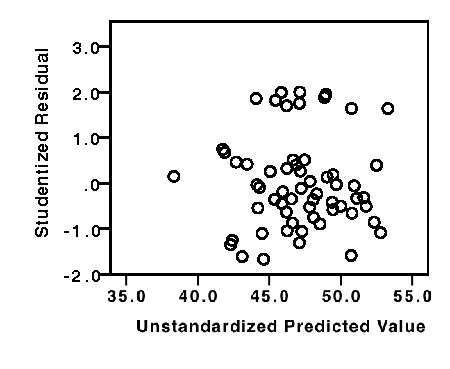
\includegraphics[width=\textwidth]{images/linearity/ValMax.eps}
    \caption{Related to test of valence, maximum pressure, and duration}
    \label{fig:valence_maximum}
\end{subfigure}
\quad
\begin{subfigure}[b]{0.45\textwidth}
    \centering
    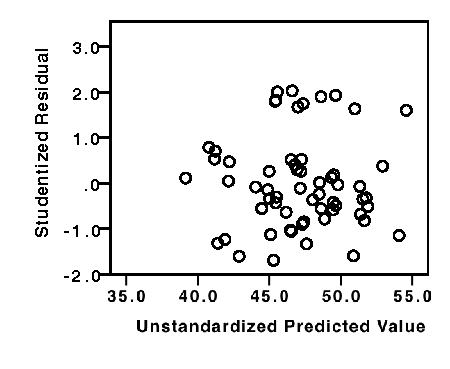
\includegraphics[width=\textwidth]{images/linearity/ValAvg.eps}
    \caption{Related to test of valence, average pressure, and duration}
    \label{fig:valence_avg}
\end{subfigure}
\par\bigskip
\par\bigskip
\begin{subfigure}[b]{0.45\textwidth}
    \centering
    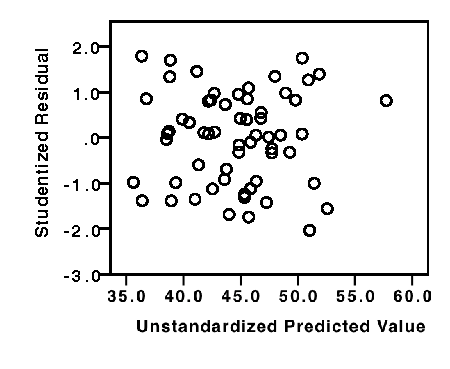
\includegraphics[width=\textwidth]{images/linearity/ArMax.eps}
    \caption{Related to test of arousal, maximum pressure, and duration}
    \label{fig:arousal_maximum}
\end{subfigure}
\quad
\begin{subfigure}[b]{0.45\textwidth}
    \centering
    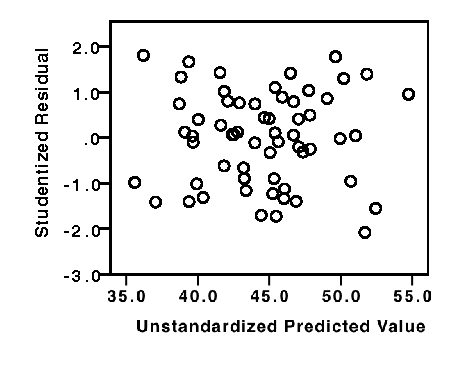
\includegraphics[width=\textwidth]{images/linearity/ArAvg.eps}
    \caption{Related to test of arousal, average pressure, and duration}
    \label{fig:arousal_avg}
\end{subfigure}
\caption{Scatter plots of predicted values against studentitized residuals. Note that because of random nature, linearity can still be assumed.}
\end{figure}
\clearpage

\subsection{Partial regression plots}
\hfill \break
%!TEX root = ../Thesis.tex
\begin{figure}[ht]
  \centering
  \begin{subfigure}[b]{0.45\textwidth}
    \centering
    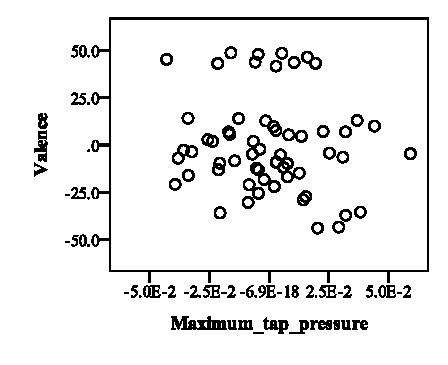
\includegraphics[width=\textwidth]{images/linearity/partialregression/valence/ValMaxMax.eps}
    \label{fig:valmaxmax}
  \end{subfigure}
  \quad
  \begin{subfigure}[b]{0.45\textwidth}
    \centering
    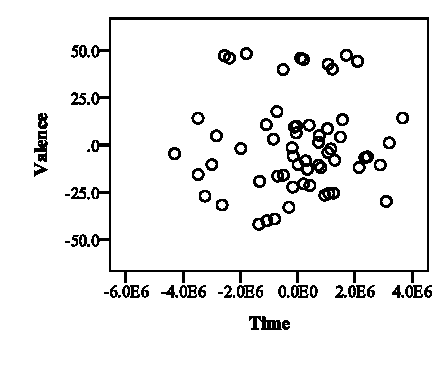
\includegraphics[width=\textwidth]{images/linearity/partialregression/valence/ValMaxTime.eps}
    \label{fig:valmaxtime}
  \end{subfigure}
  \caption{Partial regression plots with valence (dependent variable), maximum pressure and duration (independent variables). Note the approximate linearity.}
\end{figure}

\begin{figure}[ht]
  \centering
  \begin{subfigure}[b]{0.45\textwidth}
    \centering
    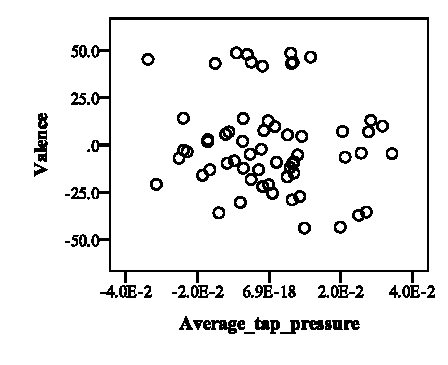
\includegraphics[width=\textwidth]{images/linearity/partialregression/valence/ValAvgAvg.eps}
    \label{fig:valavgavg}
  \end{subfigure}
  \quad
  \begin{subfigure}[b]{0.45\textwidth}
    \centering
    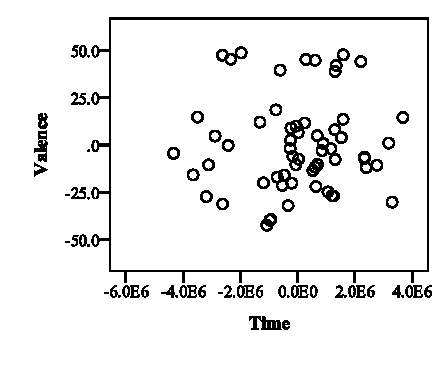
\includegraphics[width=\textwidth]{images/linearity/partialregression/valence/ValAvgTime.eps}
    \label{fig:valavgtime}
  \end{subfigure}
  \caption{Partial regression plots with valence (dependent variable), average pressure and duration (independent variables). Note the approximate linearity.}
\end{figure}
%!TEX root = ../Thesis.tex
\begin{figure}[ht]
  \centering
  \begin{subfigure}[b]{0.45\textwidth}
    \centering
    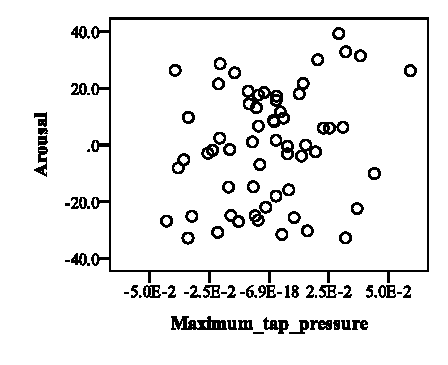
\includegraphics[width=\textwidth]{images/linearity/partialregression/arousal/ArMaxMax.eps}
    \label{fig:armaxmax}
  \end{subfigure}
  \quad
  \begin{subfigure}[b]{0.45\textwidth}
    \centering
    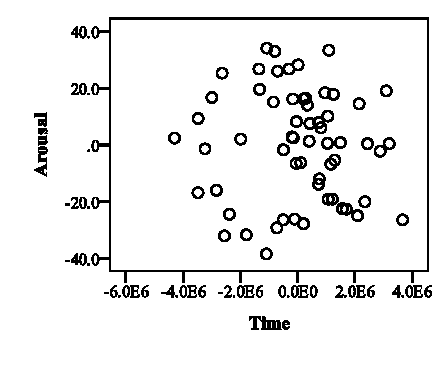
\includegraphics[width=\textwidth]{images/linearity/partialregression/arousal/ArMaxTime.eps}
    \label{fig:armaxtime}
  \end{subfigure}
  \caption{Partial regression plots with arousal (dependent variable), maximum pressure and duration (independent variables). Note the approximate linearity.}
\end{figure}

\begin{figure}[ht]
  \centering
  \begin{subfigure}[b]{0.45\textwidth}
    \centering
    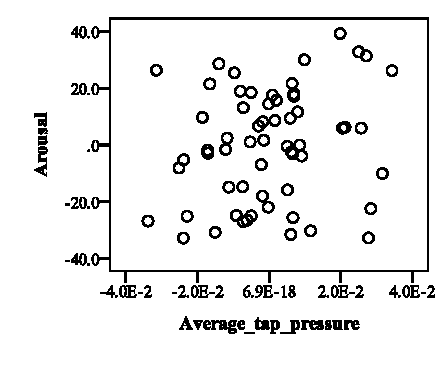
\includegraphics[width=\textwidth]{images/linearity/partialregression/arousal/ArAvgAvg.eps}
    \label{fig:aravgavg}
  \end{subfigure}
  \quad
  \begin{subfigure}[b]{0.45\textwidth}
    \centering
    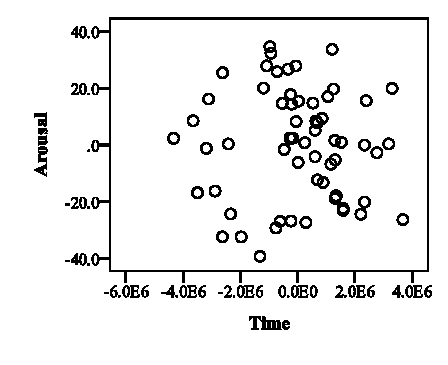
\includegraphics[width=\textwidth]{images/linearity/partialregression/arousal/ArAvgTime.eps}
    \label{fig:aravgtime}
  \end{subfigure}
  \caption{Partial regression plots with arousal (dependent variable), average pressure and duration (independent variables). Note the approximate linearity.}
\end{figure}
\clearpage

\section{Multicollinearity} % (fold)
\label{app:multicollinearity}
\hfill \break
%!TEX root=../Thesis.tex
\begin{table}[ht]
\centering
\begin{tabular}{@{}llrrr@{}}
                    &                   & Valence & Duration & Max. tap pressure \\ \midrule
Pearson Correlation & Valence           & 1.000   & -.028    & -.120             \\
                    & Duration          & -.028   & 1.000    & .522              \\
                    & Max. tap pressure & -.120   & .522     & 1.000             \\ \midrule
Sig. (1-tailed)     & Valence           & .       & .415     & .181              \\
                    & Duration          & .415    & .        & .000              \\
                    & Max. tap pressure & .181    & .000     & .                
\end{tabular}
\caption{Correlations of valence, maximum tap pressure and duration.}
\label{tab:correlations_valmax}
\end{table}

\par\bigskip

\begin{table}[ht]
\centering
\begin{tabular}{@{}llrrr@{}}
                    &                   & Valence & Duration & Avg. tap pressure \\ \midrule
Pearson Correlation & Valence           & 1.000   & -.028    & -.132             \\
                    & Duration          & -.028   & 1.000    & .492              \\
                    & Avg. tap pressure & -.132   & .492     & 1.000             \\ \midrule
Sig. (1-tailed)     & Valence           & .       & .415     & .158              \\
                    & Duration          & .415    & .        & .000              \\
                    & Avg. tap pressure & .158    & .000     & .                
\end{tabular}
\caption{Correlations of valence, average tap pressure and duration}
\label{tab:correlations_valavg}
\end{table}

\par\bigskip

\begin{table}[ht]
\centering
\begin{tabular}{@{}llrrr@{}}
                    &                   & Arousal & Duration & Max. tap pressure \\ \midrule
Pearson Correlation & Arousal           & 1.000   & .080     & .228              \\
                    & Duration          & .080    & 1.000    & .522              \\
                    & Max. tap pressure & .228    & .522     & 1.000             \\ \midrule
Sig. (1-tailed)     & Arousal           & .       & .272     & .040              \\
                    & Duration          & .272    & .        & .000              \\
                    & Max. tap pressure & .040    & .000     & .                
\end{tabular}
\caption{Correlations of arousal, maximum tap pressure and duration}
\label{tab:correlations_armax}
\end{table}

\par\bigskip

\begin{table}[!htbp]
\centering
\begin{tabular}{@{}llrrr@{}}
                    &                   & Arousal & Duration & Avg. tap pressure \\ \midrule
Pearson Correlation & Arousal           & 1.000   & .080     & .212              \\
                    & Duration          & .080    & 1.000    & .492              \\
                    & Avg. tap pressure & .212    & .492     & 1.000             \\ \midrule
Sig. (1-tailed)     & Arousal           & .       & .272     & .052              \\
                    & Duration          & .272    & .        & .000              \\
                    & Avg. tap pressure & .052    & .000     & .                
\end{tabular}
\caption{Correlations of arousal, average tap pressure and duration}
\label{tab:correlations_aravg}
\end{table}
\clearpage
% section multicollinearity (end)

\section{Unusual data points} % (fold)
\label{sec:unusual_data_points}
\hfill \break
%!TEX root=../Thesis.tex
% Please add the following required packages to your document preamble:
% \usepackage{booktabs}
\begin{table}[h]
\centering
\begin{tabularx}{\textwidth}{@{}llZZZZZZ@{}}
\textbf{Dependent variable} & \textbf{Independent variables} & \multicolumn{2}{c}{\textbf{Studentized residuals}}  & \multicolumn{2}{c}{\textbf{Cook's Distance}}        & \multicolumn{2}{c}{\textbf{Leverage values}}        \\ \midrule
                            &                                & \multicolumn{1}{r}{Min} & \multicolumn{1}{r}{Max} & \multicolumn{1}{r}{Min} & \multicolumn{1}{r}{Max} & \multicolumn{1}{r}{Min} & \multicolumn{1}{r}{Max} \\ \cmidrule(l){3-8} 
Valence                     & Max. tap pressure, duration    & -1.7                     & 2.06                     & .0                       & .09                      & .0                       & .14                      \\
                            & Avg. tap pressure, duration    & -1.72                    & 2.09                     & .0                       & .09                      & .0                       & .1                       \\ \midrule
Arousal                     & Max. tap pressure, duration    & -2.1                     & 1.83                     & .0                       & .08                      & .0                       & .14                      \\
                            & Avg. tap pressure, duration    & -2.15                    & 1.84                     & .0                       & .11                      & .0                       & .1                      
\end{tabularx}
\caption{Studentized residuals, Cook's values and leverage values. Studentized residuals are between -3 and +3 SDs. Cook's Distance values are $< 1$. Leverage values are $< .2$.}
\label{tab:unusual_data_points}
\end{table}
\clearpage
% section unusual_data_points (end)

\section{Normality} % (fold)
\label{app:normality}
\hfill \break
%!TEX root=../Thesis.tex
\begin{figure}[ht]
\centering
\begin{subfigure}[b]{0.45\textwidth}
    \centering
    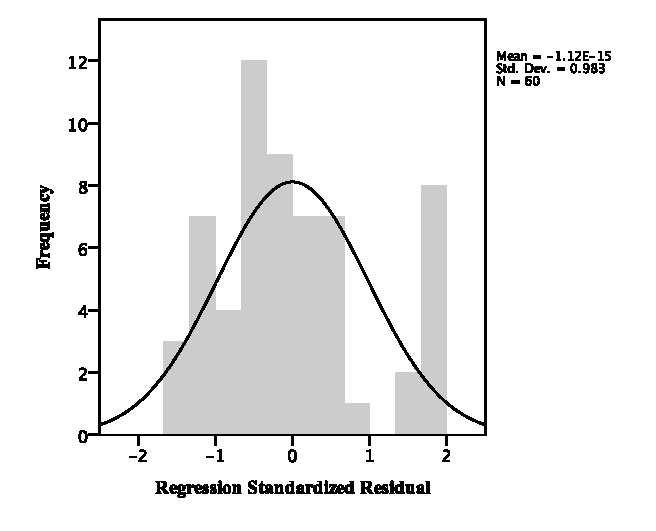
\includegraphics[width=\textwidth]{images/normality/ValMax/HistValMax.eps}
    \caption{Histogram}
    \label{fig:histvalmax}
\end{subfigure}
\quad
\begin{subfigure}[b]{0.45\textwidth}
    \centering
    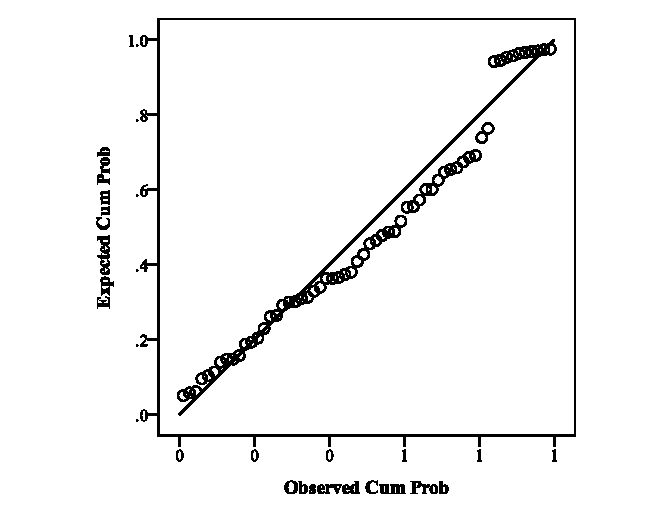
\includegraphics[width=\textwidth]{images/normality/ValMax/PPValMax.eps}
    \caption{P-P plot}
    \label{fig:ppvalmax}
\end{subfigure}
\caption{Normality graphs for valence, maximum tap pressure and duration.}
\end{figure}
\par\bigskip
\par\bigskip
\begin{figure}[ht]
\centering
\begin{subfigure}[b]{0.45\textwidth}
    \centering
    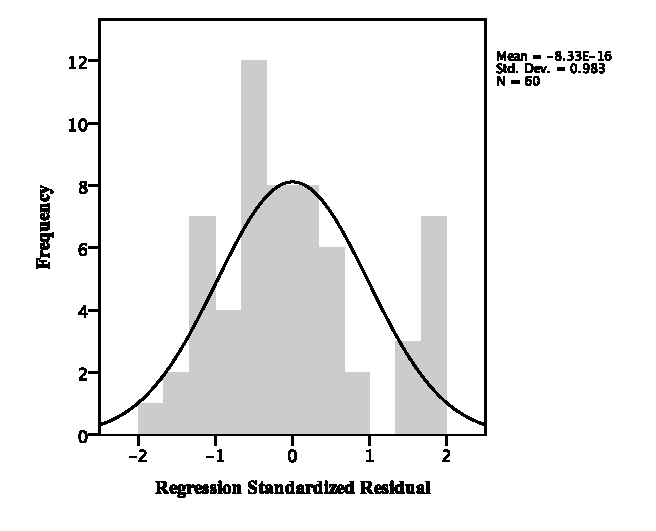
\includegraphics[width=\textwidth]{images/normality/valavg/HistValAvg.eps}
    \caption{Histogram}
    \label{fig:histvalavg}
\end{subfigure}
\quad
\begin{subfigure}[b]{0.45\textwidth}
    \centering
    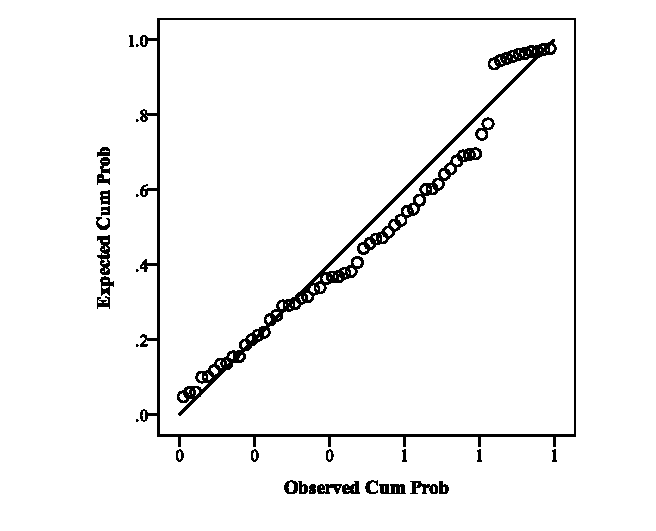
\includegraphics[width=\textwidth]{images/normality/valavg/PPValAvg.eps}
    \caption{P-P plot}
    \label{fig:ppvalavg}
\end{subfigure}
\caption{Normality graphs for valence, average tap pressure and duration.}
\end{figure}
\par\bigskip
\par\bigskip
\begin{figure}[ht]
\centering
\begin{subfigure}[b]{0.45\textwidth}
    \centering
    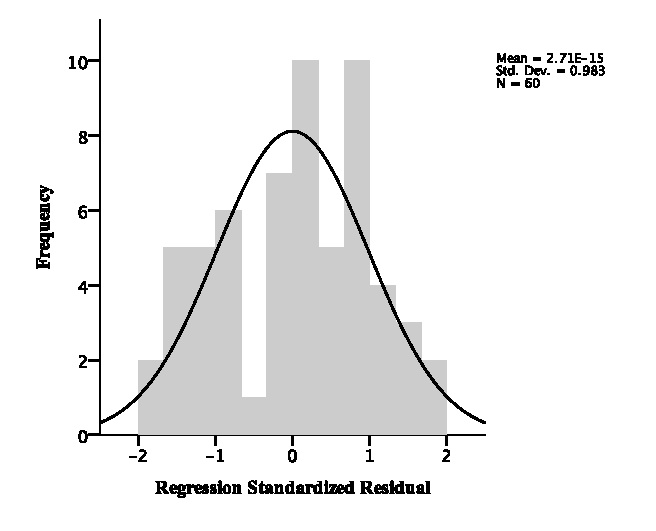
\includegraphics[width=\textwidth]{images/normality/ArMax/HistArMax.eps}
    \caption{Histogram}
    \label{fig:histarmax}
\end{subfigure}
\quad
\begin{subfigure}[b]{0.45\textwidth}
    \centering
    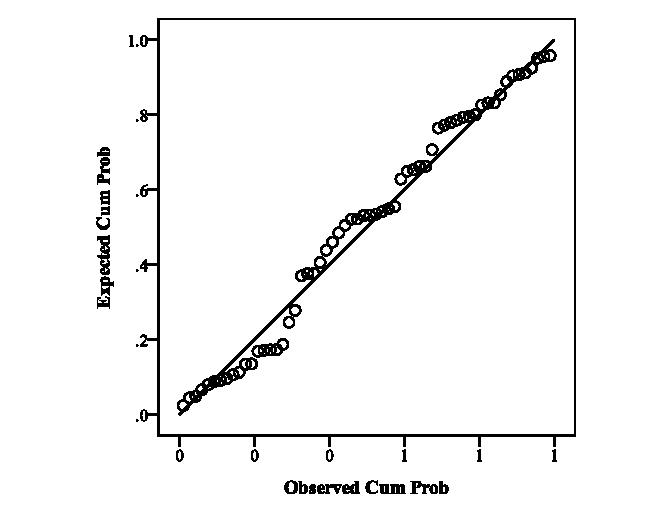
\includegraphics[width=\textwidth]{images/normality/ArMax/PPArMax.eps}
    \caption{P-P plot}
    \label{fig:pparmax}
\end{subfigure}
\caption{Normality graphs for arousal, average tap pressure and duration.}
\end{figure}
\par\bigskip
\par\bigskip
\begin{figure}[ht]
\centering
\begin{subfigure}[b]{0.45\textwidth}
    \centering
    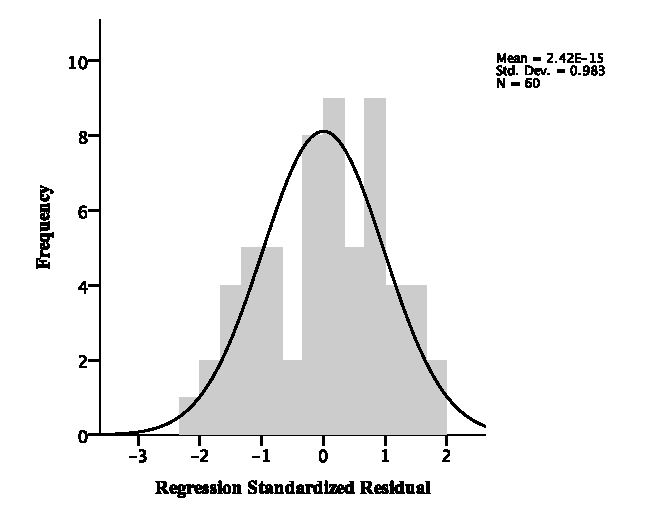
\includegraphics[width=\textwidth]{images/normality/aravg/HistArAvg.eps}
    \caption{Histogram}
    \label{fig:histaravg}
\end{subfigure}
\quad
\begin{subfigure}[b]{0.45\textwidth}
    \centering
    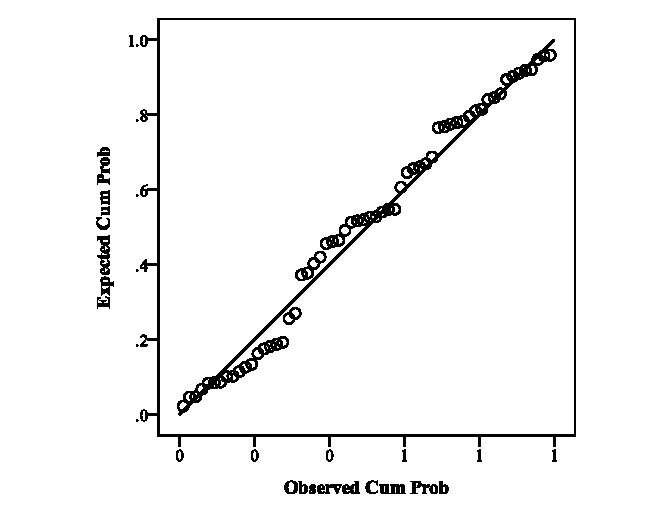
\includegraphics[width=\textwidth]{images/normality/aravg/PPArAvg.eps}
    \caption{P-P plot}
    \label{fig:pparavg}
\end{subfigure}
\caption{Normality graphs for arousal, average tap pressure and duration.}
\end{figure}
\clearpage
% section normality (end)

\section{Regression coefficients} % (fold)
\label{sec:regression_coefficients}
\hfill \break
%!TEX root=../Thesis.tex
\begin{table}[ht]
\centering
\begin{tabularx}{\textwidth}{@{}llZZZZ@{}}
\textbf{Dependent variable} & \textbf{Independent variable*} & B              & $SE_b$  & $\beta$ & \textit{Significance} \\ \midrule
Valence                     & Intercept                      & 53.722         & 139.848 & n.a.    & .702                  \\
                            & Max. tap pressure              & -136.476       & 145.694 & -.144   & .353                  \\
                            & Duration                       & $5.566e^{-7}$  & .000    & .047    & .761                  \\ \cmidrule(l){2-6} 
                            & Intercept                      & 59.459         & 138.468 & n.a.    & .669                  \\
                            & Avg. tap pressure              & -211.353       & 204.722 & -.156   & .306                  \\
                            & Duration                       & $5.698e^{-7}$  & .000    & .048    & .750                  \\ \midrule
Arousal                     & Intercept                      & 10.397         & 109.668 & n.a.    & .925                  \\
                            & Max. tap pressure              & 193.809        & 114.182 & .256    & .095                  \\
                            & Duration                       & $-5.1e^{-7}$   & .000    & -.054   & .722                  \\ \cmidrule(l){2-6} 
                            & Intercept                      & -2.076         & 109.254 & n.a.    & .985                  \\
                            & Avg. tap pressure              & 247.231        & 161.530 & .227    & .131                  \\
                            & Duration                       & $-3.027e^{-7}$ & .000    & -.032   & .830                 
\end{tabularx}
\caption{Regression coefficients table with significance. \textit{B} = Unstandardized coefficient. \textit{$SE_b$} = Std. Error. \textit{$\beta$} = Standardized coefficients. Significance = p-value. *\textit{Note}: Intercept should not be regarded as independent variable.}
\label{tab:regression_coefficients}
\end{table}
\clearpage
% section regression_coefficients (end)

\section{Secondary study - Linearity}
\label{app:sec_linearity}
\hfill \break
%!TEX root=../Thesis.tex
\begin{figure}[ht]
\centering
\begin{subfigure}[b]{0.45\textwidth}
    \centering
    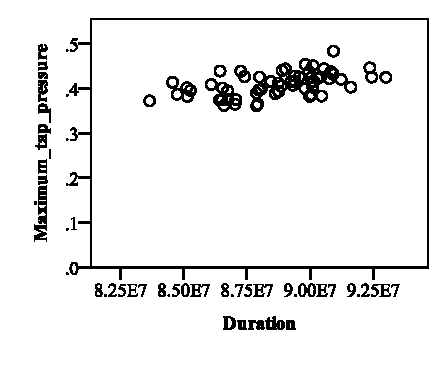
\includegraphics[width=\textwidth]{images/secondary/max/MaxLinearity.eps}
    \label{fig:sec_max_lin}
\end{subfigure}
\quad
\begin{subfigure}[b]{0.45\textwidth}
    \centering
    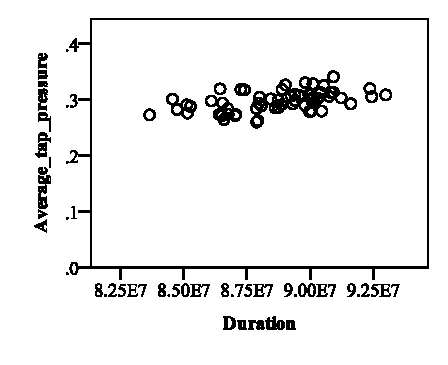
\includegraphics[width=\textwidth]{images/secondary/avg/AvgLinearity.eps}
    \label{fig:sec_avg_lin}
\end{subfigure}
\caption{Linearity assessment graphs for max. tap pressure (left) and avg. tap pressure (right). It shows a scatter plot of tap pressure against tap duration. Both graphs show a strong sign of linearity.}
\end{figure}
\clearpage

\section{Secondary study - Normality} % (fold)
\label{sec:sec_normality}
\hfill \break
%!TEX root=../Thesis.tex
\begin{figure}[ht]
\centering
\begin{subfigure}[b]{0.45\textwidth}
    \centering
    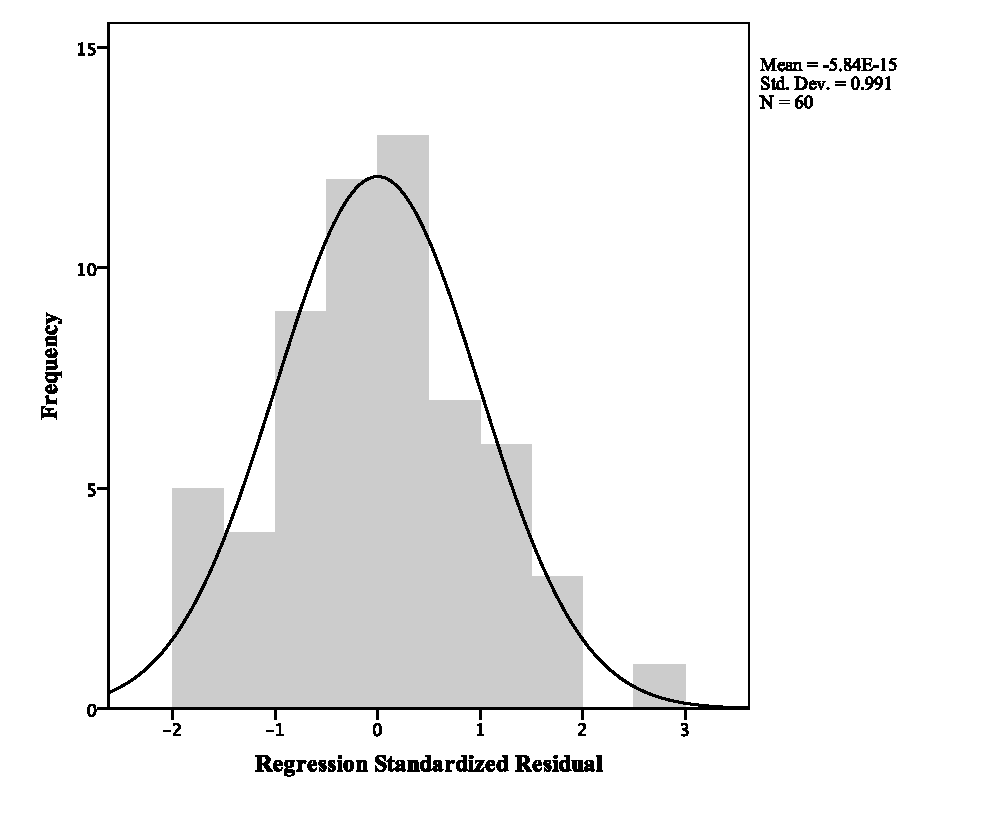
\includegraphics[width=\textwidth]{images/secondary/max/MaxHistogram.eps}
    \caption{Histogram}
    \label{fig:sec_max_hist}
\end{subfigure}
\quad
\begin{subfigure}[b]{0.45\textwidth}
    \centering
    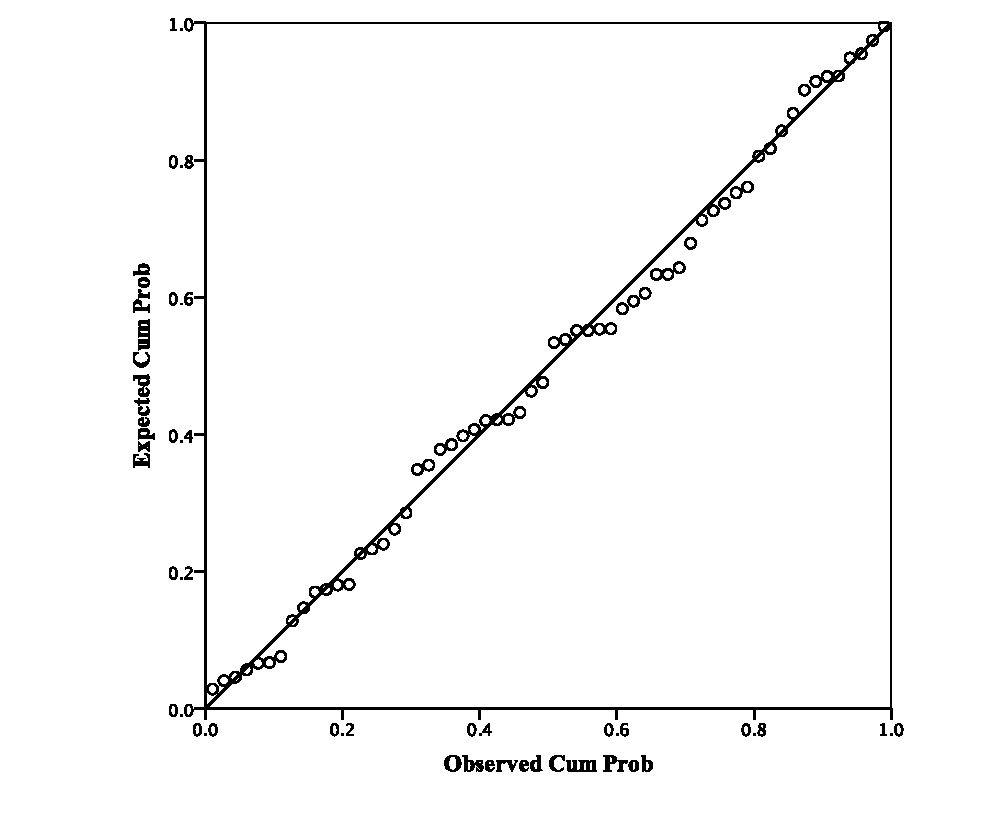
\includegraphics[width=\textwidth]{images/secondary/max/MaxP-P.eps}
    \caption{P-P plot}
    \label{fig:sec_max_PP}
\end{subfigure}
\caption{Normality graphs for max. tap pressure and duration. The histogram shows an approximate normal distribution. The P-P plot shows little deviation from the origin line, further proving a normal distribution of samples.}
\end{figure}
\par\bigskip
\par\bigskip
\begin{figure}[ht]
\begin{subfigure}[b]{0.45\textwidth}
    \centering
    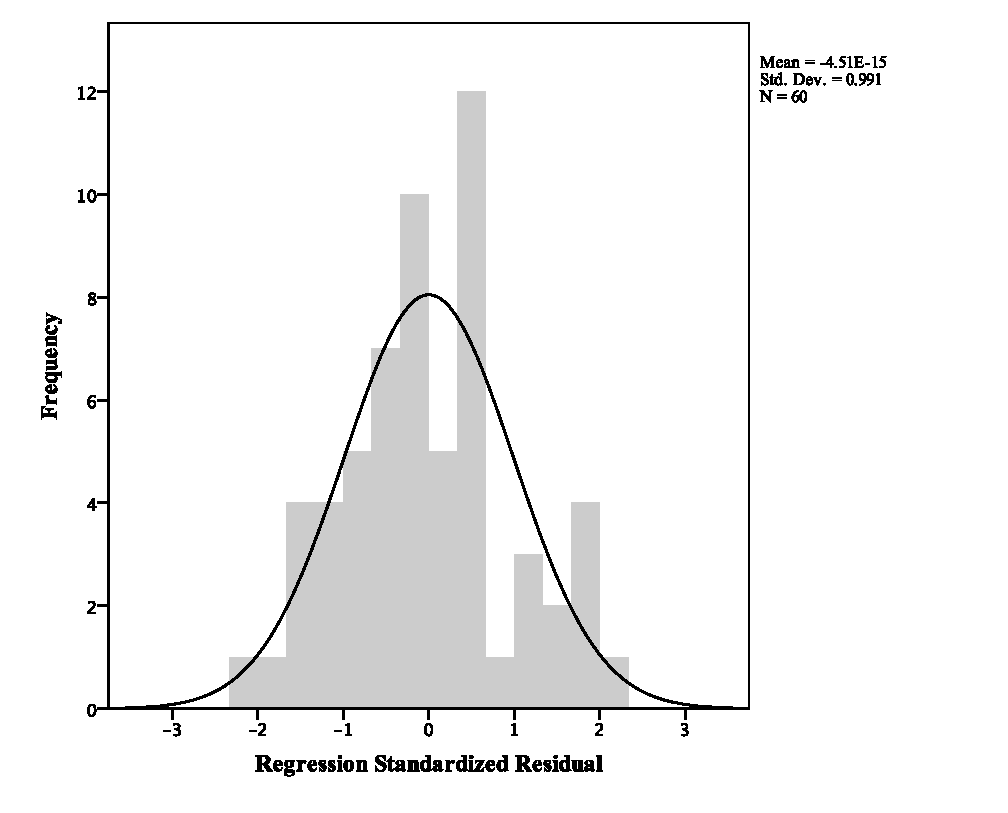
\includegraphics[width=\textwidth]{images/secondary/avg/AvgHistogram.eps}
    \caption{Histogram}
    \label{fig:sec_avg_hist}
\end{subfigure}
\quad
\begin{subfigure}[b]{0.45\textwidth}
    \centering
    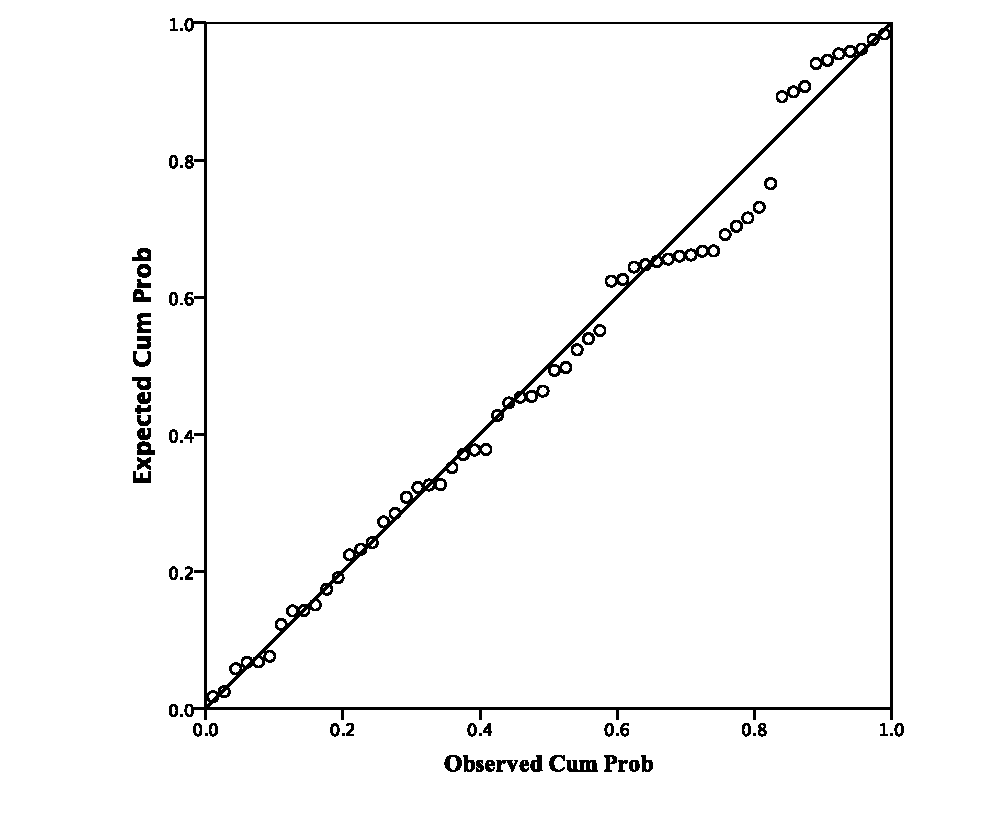
\includegraphics[width=\textwidth]{images/secondary/avg/AvgP-P.eps}
    \caption{P-P plot}
    \label{fig:sec_avg_PP}
\end{subfigure}
\caption{Normality graphs for avg. tap pressure and duration. The histogram shows an approximate normal distribution. The P-P plot shows little deviation from the origin line except at the top right, where it deviates a little more. Still, the deviation is not large enough to warrant any concerns over normal distribution of samples.}
\end{figure}
\clearpage

\section{Secondary study - Regression coefficients}
\label{sec:sec_regression_coefficients}
\hfill \break
%!TEX root=../Thesis.tex
\begin{table}[ht]
\centering
\begin{tabularx}{0.8\textwidth}{@{}llZZZZ@{}}
\textbf{Dependent variable} & \textbf{Independent variable*} & B             & $SE_b$ & $\beta$ & \textit{Significance} \\ \midrule
Max. tap pressure           & Intercept                      & -.169         & .124   & n.a.    & .180                  \\
                            & Duration                       & $6.552e^{-9}$ & .000   & .522    & $> .0005$             \\ \midrule
Avg. tap pressure           & Intercept                      & -.082         & .088   & n.a.    & .357                  \\
                            & Duration                       & $4.274e^{-9}$ & .000   & .492    & $> .0005$            
\end{tabularx}
\caption{Regression coefficients table with significance. \textit{B} = Unstandardized coefficient. \textit{$SE_b$} = Std. Error. \textit{$\beta$} = Standardized coefficients. Significance = p-value. *\textit{Note}: Intercept should not be regarded as independent variable.}
\label{tab:secondary_regression_coefficients}
\end{table}
\clearpage


% section secondary_study_results (end)


\end{document}

%%% Local Variables:
%%% mode: latex
%%% TeX-master: t
%%% End:
